\documentclass{IEEEtran}

\special{papersize=8.5in,11in}
\usepackage{amsmath}
\usepackage{amssymb}
\usepackage{mathptm}
\usepackage{url}
\usepackage{times}
\usepackage{graphicx,color}
\usepackage{CJKutf8}
\usepackage{multirow}
\usepackage{kotex}
\usepackage{gensymb}
%\usepackage{stfloats}
\usepackage[labelformat=simple]{subcaption}
\renewcommand\thesubfigure{(\alph{subfigure})}

\setlength{\emergencystretch}{2em}
\setlength{\parindent}{0em}

\begin{document}

\title{Runtime Power Management of Battery Electric Vehicles for Extended Range with Consideration of Driving Time}

\author{
Donkyu~Baek,~\IEEEmembership{Member,~IEEE,}
Jaemin~Kim,~\IEEEmembership{Member,~Student IEEE} and
Naehyuck~Chang,~\IEEEmembership{Fellow,~IEEE}

\thanks{Direct questions and comments about this article to Naehyuck Chang, Korea Advanced Institute of Science and Technology, 291, Daehak-ro, Yuseong-gu, Daejeon, Korea (e-mail: naehyuck@cad4x.kaist.ac.kr). This work is supported in part by NRF Grant 2015R1A2A1A09005694.}
}

\maketitle

%% I replace "the minimum-energy-velocity planning" with "energy-aware-velocity planning" because this paper does not pursuit the minimum energy but the minimum EDP.
%% However, DO NOT mechanically change the minimum-energy with energy-aware. Section 4B Line 3 for example, it should be minimum-energy. 
%% I modified the minimum-energy constant with least-energy. 

\begin{abstract}
Installation of a large-capacity battery pack is a straightforward method to extend the range of battery-electric vehicles (BEV, or all-electric vehicles). However, at the same time, a large-capacity battery pack not only occupies a big space but significantly increases the vehicle weight, which directly impacts on the fuel economy and vehicle performance. This implies that increasing the battery capacity has an obvious limitation in extending the EV range. 
In this paper, we introduce a system-level framework to extend the range of BEV with the consideration of the vehicle dynamics, electric powertrain characteristics, road slopes, payload, and regenerative braking. This work particularly takes into account driving time so that the resultant BEV power management does not impractically slow down the vehicle velocity. 

The BEV power management framework derives \textit{energy-aware-velocity planning}, i.e., a desirable instantaneous velocity at each distance step (or at each time instant). The major technical contributions of this paper compared with the previous work include i) practically applicable velocity planning for production BEVs from superb BEV power model fidelity, ii) new performance metrics to consider both driving energy and driving time: energy-delay product ($EDP$), energy-square-delay product ($E^2DP$) and energy-cubic-delay product ($E^3DP$), iii) heuristics to derive $EDP$-aware-velocity planning, iv) comparative analysis of the velocity planning between BEV and internal combustion engine vehicles (ICEV), and v) analysis of the model fidelity impact on the energy-aware-velocity planning. The proposed method results in up to a 43.4\% extended range and a 51.7\% improvement of the $EDP$ compared with the least-energy-constant-velocity driving.
\end{abstract}

%%%%%%%%%%%%%%%%%%%%%%%%%%%%%%%%%%%%%%%%%%%%%
\begin{IEEEkeywords}
Electric vehicles, Battery electric vehicles, Energy-aware velocity, Range extension
\end{IEEEkeywords}
%%%%%%%%%%%%%%%%%%%%%%%%%%%%%%%%%%%%%%%%%%
\section{Introduction}
%%%%%%%%%%%%%%%%%%%%%%%%%%%%%%%%%%%%%%%%%%

Battery-electric vehicles (BEV, simply EV for the rest of the paper) stand for all-electric vehicles that are powered solely by the battery. EV owners generally have range anxiety because the fully-charged range of EV is still considerably shorter than that of internal combustion engine vehicles (ICEV.) Lack of charging facility and longer charging time make the anxiety stronger, which is comparable to vehicle breakdown.

Unfortunately, it is hard to achieve a longer range from further efficiency enhancement of the major electric powertrain components such as traction motors, power converters, batteries, and so on, because they already exhibit a high efficiency (90\% or higher), and thus the headroom for further enhancement is very narrow.

A straightforward way to extend the range is to install a larger-capacity battery. However, this method does not only cause a higher manufacturing cost but also higher daily operating cost because it  directly increases the vehicle curb weight, which is inversely proportional to the fuel economy~\cite{Hong:ASPDAC16}. Carrying a large-capacity battery also makes the passenger compartment smaller. In addition, the increased weight also directly impacts on the performance of the vehicle. 
EVs should be equipped with a more powerful drivetrain to compensate the weight increase, which again makes EV consume more energy. 
EVs deploy a large portion of light materials such as aluminum and carbon fiber to compensate the heavy battery weight, and not to degrade the fuel economy and performance significantly~\cite{Chang:ICCAD14}. However, such a way also causes a significant manufacturing and repairing cost increase because light materials that ensure strength are generally very expensive and not repairable by sheeting. These conventional ways of extending the EV range may have a negative impact on the cost of ownership.

This paper introduces a runtime power management to extend the range without increasing the cost of ownership. EV energy consumption is largely different by the cruising velocity, acceleration, weight, load slope, etc. \cite{Chang:ICCAD14}. The concept of low-energy vehicle driving comes to reduce $CO_2$ emissions from ICEV. Lower  $CO_2$ emission generally implies less fuel consumption~\cite{Seraens:thesis12}. 

However, low-energy ICEV driving results are not applicable to EVs due to significant differences 
between the engine and electric powertrain. An internal combustion engine with a transmission is a common ICEV powertrain structure while EV electric powertrain has an electric motor with a fixed ratio gearbox (a reducer.) A transmission is a mandatory component of ICEVs as the engine torque and power are distinct convex functions of the engine RPM (revolutions per minute.) On the other hand, electric motors have a flat torque from zero RPM to the base (rated) RPM. Such advantage enables passenger vehicles not to mandate a transmission as long as there is no significant variation in the payload like heavy-duty trucks and buses. A higher motor RPM over the base speed is achieved by the use of field weakening, and a single reduction ratio gearbox can exhibit a fast enough top velocity. Regenerative braking is another advantage of EVs, which fundamentally changes the vehicle power consumption when it decelerates.

In this paper, we derive the energy-aware velocity for a given EV and demonstrate its fundamental differences from that of ICEV.
We derive an analytical EV power model with a scale of production EVs such as Chevrolet  Bolt. We introduce new performance metrics for EV, energy-delay product ($EDP$), energy-square-delay product ($E^2DP$) and energy-cubic-delay product ($E^3DP$), which demonstrates a practically applicable energy-aware-velocity planning. The proposed method results in up to a 43.4\% extended driving range without increasing battery capacity, and a 51.7\% improvement of $EDP$ compared with the least-energy-constant-velocity driving. 


\textcolor{red}{We summarize the paper structure as follows. Section~\ref{sec:related work} describes related work for low-energy driving for both ICEV and EV. Section~\ref{sec:energy consumption} introduces analysis of power consumption of ICEV and EV  by the vehicle setup and driving conditions. This section also compares power consumption characteristics of EV with those of ICEV and demonstrates why  ICEV eco-driving results can hardly apply to EV. Section~\ref{sec:framework} introduces an EV specific system-level framework for energy-aware-velocity planning. In this section, we are first to introduce new single performance metrics to take into account both driving energy and driving time in this section. We visualize the impacts of the model fidelity on the energy-aware-velocity planning in Section~\ref{sec:impact_EV_power model}. Section~\ref{sec:conclusions} is a summary of major technical contribution of this paper.}
%%%%%%%%%%%%%%%%%%%%%%%%%%%%%%%%%%%%%%%%%%
\section{Related work} \label{sec:related work}
%%%%%%%%%%%%%%%%%%%%%%%%%%%%%%%%%%%%%%%%%%
  
Low-energy driving is proposed for ICEVs to assists drivers in order to save fuel consumption and reduce emissions~\cite{Seraens:thesis12, Kamal:TITS11, Ozatay:TITS14, Dovgana:ASC14, Ozatay:IFAC14, Khayyam:ESA12}.  
The fuel consumption model is a polynomial form based on a general vehicle dynamics model and takes into account the transmission shift position. 

There has been low-energy driving research for EVs as well, but previous research relies on the vehicle dynamics models such as rolling resistance, gradient resistance, aerodynamic resistance, and so forth~\cite{Yan:NAPS14}, which ignores a loss of energy transformation from electricity to mechanical energy. Such simplification makes it impossible to count on the powertrain efficiency at all, regardless of ICEV or EV. 

It has been reported that even EV power models that consider the motor loss~\cite{Lin:ICCA14, Wu:ITS15, Dib:IVPPC11} can hardly reproduce correct EV drivetrain power consumption~\cite{Hong:ASPDAC16}. This paper  demonstrates how incorrect EV power model can mislead the energy-aware-velocity planning in Section~\ref{sec:energy consumption}. 

There have been previous practices that demonstrate how EVs should change the vehicle velocity to reduce energy consumption under  a given road and traffic conditions. Such work commonly formulates an offline optimization problem and uses a dynamic programming (DP) to derive the globally optimal solution~\cite{Lin:ICCA14, Dib:IVPPC11, Dib:OGST12, Mensing:TR13}. However, once again, such work usually uses the vehicle dynamics model for the EV power model. It borrows the parameters from commercial vehicles such as the vehicle curb weight, aerodynamic resistance from the vehicle specifications and the rolling resistance from the tire specifications~\cite{Lin:ICCA14}. 

An empirical modeling has a potential to achieve more accurate power model  of a particular target EV. Related work fabricates a custom EV, collects the GPS tracking, battery voltage and battery current and constructs an EV power consumption model with several parameters~\cite{Dib:IVPPC11}. However, this power model still has important parameters missing that significantly affect the model fidelity such as friction loss, iron loss and windage loss in the motor, loss in the drivetrain and regenerative braking. Inaccurate EV power consumption model misleads the energy-aware-velocity planning. A more recent work fabricates a low-speed custom EV and derived an accurate power model. The power model reflects various EV-specific factors including regenerative braking and even for drivetrain loss by regression analysis of a large amount of driving data. However, the power model is limited to low-speed EVs and hard to accommodate production EVs~\cite{Hong:ASPDAC16}. 

Some work attempts to accommodate more realistic driving conditions such as traffic signals and stop signs. However, the results are lack of practicality due to the assumption of a constant road slope and a constant cruising velocity with highly simplified EV power models~\cite{Yan:NAPS14, Dib:CEP14, Wu:ITS15}. 

%%%%%%%%%%%%%%%%%%%%%%
%Related work
We recently see a new initiative that attempts to reduce the energy consumption of cyber-physical systems using application-aware cross-layer management. Such approaches apply algorithms, tools and methodologies relevant to design automation and embedded low-power systems~\cite{Seshia:TCAD17}. 
% Energy management 
Just naming several for instance, energy management for EV also considers drivers' behaviors and related EV power consumption to extend range~\cite{Vatanparvar:TSG18,Vatanparvar:TODAES17}.
% EV battery pack 
Electric vehicle battery packs consist of a large number of battery cells, and it is crucial to optimize the battery pack architectures in terms of capacity, cost and reliability~\cite{Wu:TCAD13,Shaheer:RTCSA17}. 
Electric vehicle battery management systems must be able to accommodate multi-power sources, provide a good scalability, and mitigate cell-to-cell variability~\cite{Shin:TCAD15}.
% Non-propulsion power
Electric vehicles consume a non-negligible amount of battery energy for non-driving power components. The related study tries to optimize energy for heating, ventilation and air conditioning (HVAC) systems equipped with electric vehicles~\cite{Zhao:ICCAD15,Vatanparvar:TECS18}. 
% Energy 
A renewable energy aware pricing scheme minimizes both the community-wide electricity bill and individual electricity bill~\cite{Liu:TPDS17}.
% HESS
A hybrid energy storage systems improve efficiency and lifetime without significant increase of the cost~\cite{Xie:TCAD13, Kim:JPS14}. 
%%%%%%%%%%%%%%%%%%%%%%




%%%%%%%%%%%%%%%%%%%%%%%%%%%%%%%%%%%%%%%%%%
\section{Vehicle Power and Energy Consumption Analysis} \label{sec:energy consumption}
%%%%%%%%%%%%%%%%%%%%%%%%%%%%%%%%%%%%%%%%%%

%%%%%%%%%%%%%%%%%%%%%%%%%%%%%%%%%%%%%%%%%%
\subsection{The least-energy-constant velocity for cruising} \label{subsec:opt-cruising}

A commonly used vehicle power consumption model is from the vehicle dynamics equation~(\ref{eq:dynamics_model}). This model considers the traction force only assuming a 100\% efficiency of the powertrain (engines, electric motors or both.) Therefore, this model is applicable to any sort of vehicles but not able to explain EV-specific power consumption.
%
\begin{equation}  \label{eq:dynamics_model} %equation 1
\begin{split}
P_{trac}	&= F \frac{ds}{dt} = Fv= (F_{R} + F_{G} + F_{I} + F_{A}) v \\
F_{R} \propto C_{rr}W,~F_{G} &\propto Wsin\theta,~F_{I} \propto ma,~\text{and}~F_{A} \propto \frac{1}{2} \rho C_d Av^2 \\
P_{trac} &\approx (\alpha  + \beta sin\theta + \gamma a + \delta v^2)mv
\end{split}
\end{equation}
where $F_R$, $F_G$, $F_I$, $F_A$, and $F_B$ denote the rolling resistance, gradient resistance, inertia resistance, aerodynamic resistance, and brake force provided by hydraulic brakes, respectively~\cite{Park:DAC13}. The coefficients $\alpha$, $\beta$, $\gamma$, and $\delta$ correspond to the rolling resistance, gradient resistance, inertia resistance, and aerodynamic resistance, respectively.

The actual power consumption evaluation of ICEV, i.e., fuel consumption rate, should take into account the powertrain efficiency. A simplified model of ICEV fuel consumption in~\cite{Kamal:TITS11} is written as follows:
%
\begin{equation} \label{eq:power_ICEV} %equation 2
P_{ICEV} = \frac{P_{trac} + P_{start}}{\eta_{ICEV}} 
\end{equation}
where $P_{start}$ is power consumption of the engine during idling. The engine efficiency, $\eta_{ICEV}$, is determined by the gear ratio, engine speed and engine torque. The gear ratio generally dynamically changes by transmission shift. The engine efficiency is generally not simple enough to explain by analytic functions and often described as efficiency maps~\cite{Kamal:TITS11}.

Adding a traction motor power model in (\ref{eq:power_ICEV}) makes (\ref{eq:dynamics_model}) and (\ref{eq:power_ICEV}) reflect more realistic EV power consumption characteristics. 
%
\begin{equation} \label{eq:motorloss_model} %equation 3
P_{EV} = \frac{P_{trac}}{\eta_{EV}}
\end{equation}
\begin{equation}
\eta_{EV} = \frac{P_{trac}}{{P_{trac} + k_c T^2 + k_i \omega + k_w \omega^3 + C}}\nonumber 
\end{equation}
where $k_c$, $T$, $k_i$, $\omega$, $k_w$, $C$ represent a copper loss coefficient, a motor torque, a coefficient by iron and friction loss, an angular speed, a windage coefficient, and constant loss, respectively~\cite{Hong:ASPDAC16}.

EVs mostly use regenerative braking during deceleration, which converts kinetic energy to electric energy except low-cost golf carts. The harvested energy from regenerative braking is closely related to the electromagnetic flux inside of the motor, and the flux is proportional to the motor RPM. The regenerative braking model of an EV can be  simplified as (\ref{eq:regen_model}) 
%
\begin{equation}\label{eq:regen_model} 
P_{regen} = \epsilon T v + \zeta
\end{equation}  %equation 4
%
where $\epsilon$ and $\zeta$ are regenerative braking coefficients.

The power consumption model (\ref{eq:motorloss_model}) is commonly used in various analytical EV power managements~\cite{Dib:IVPPC11, Dib:CEP14, Wu:TR15}. However, there are still considerable sources of power loss from  the drivetrain. To make a long story short, (\ref{eq:dynamics_model}) -- (\ref{eq:motorloss_model}) do not accurately explain EV-specific power consumption in various driving conditions according to our intensive measurement with real EVs. 

In this paper, therefore, we borrow an EV-specific power ($EV^*$) modeling method considering the loss in EV drivetrain using a multivariable regression method from the measured power data and achieve a polynomial fitting~\cite{Hong:ASPDAC16}. However, we should not directly use this power model because the model covers only low-speed EVs, i.e., slower than 35 km/h. Thus, we derive our own model coefficients in this paper.
%
\begin{equation} \label{eq:EV_specific_model} %equation 5
P_{EV^*} = \frac{P_{trac}}{\eta_{EV^*}}
\end{equation} 
\begin{equation}
\eta_{EV^*} = \frac{P_{trac}}{{P_{trac} + C_0 + C_1 v + C_2 v^2 + C_3 T^2}}\nonumber
\end{equation}	
where $C_0$, $C_1$, $C_2$, and $C_3$ mean coefficients for constant loss, iron and friction losses, drivetrain loss, and copper loss, respectively. Even if (\ref{eq:EV_specific_model}) has the same form as (\ref{eq:motorloss_model}), the actual coefficients become different if it reflects the characteristics of electric powertrain. 


\begin{figure*}	%Figure 2.
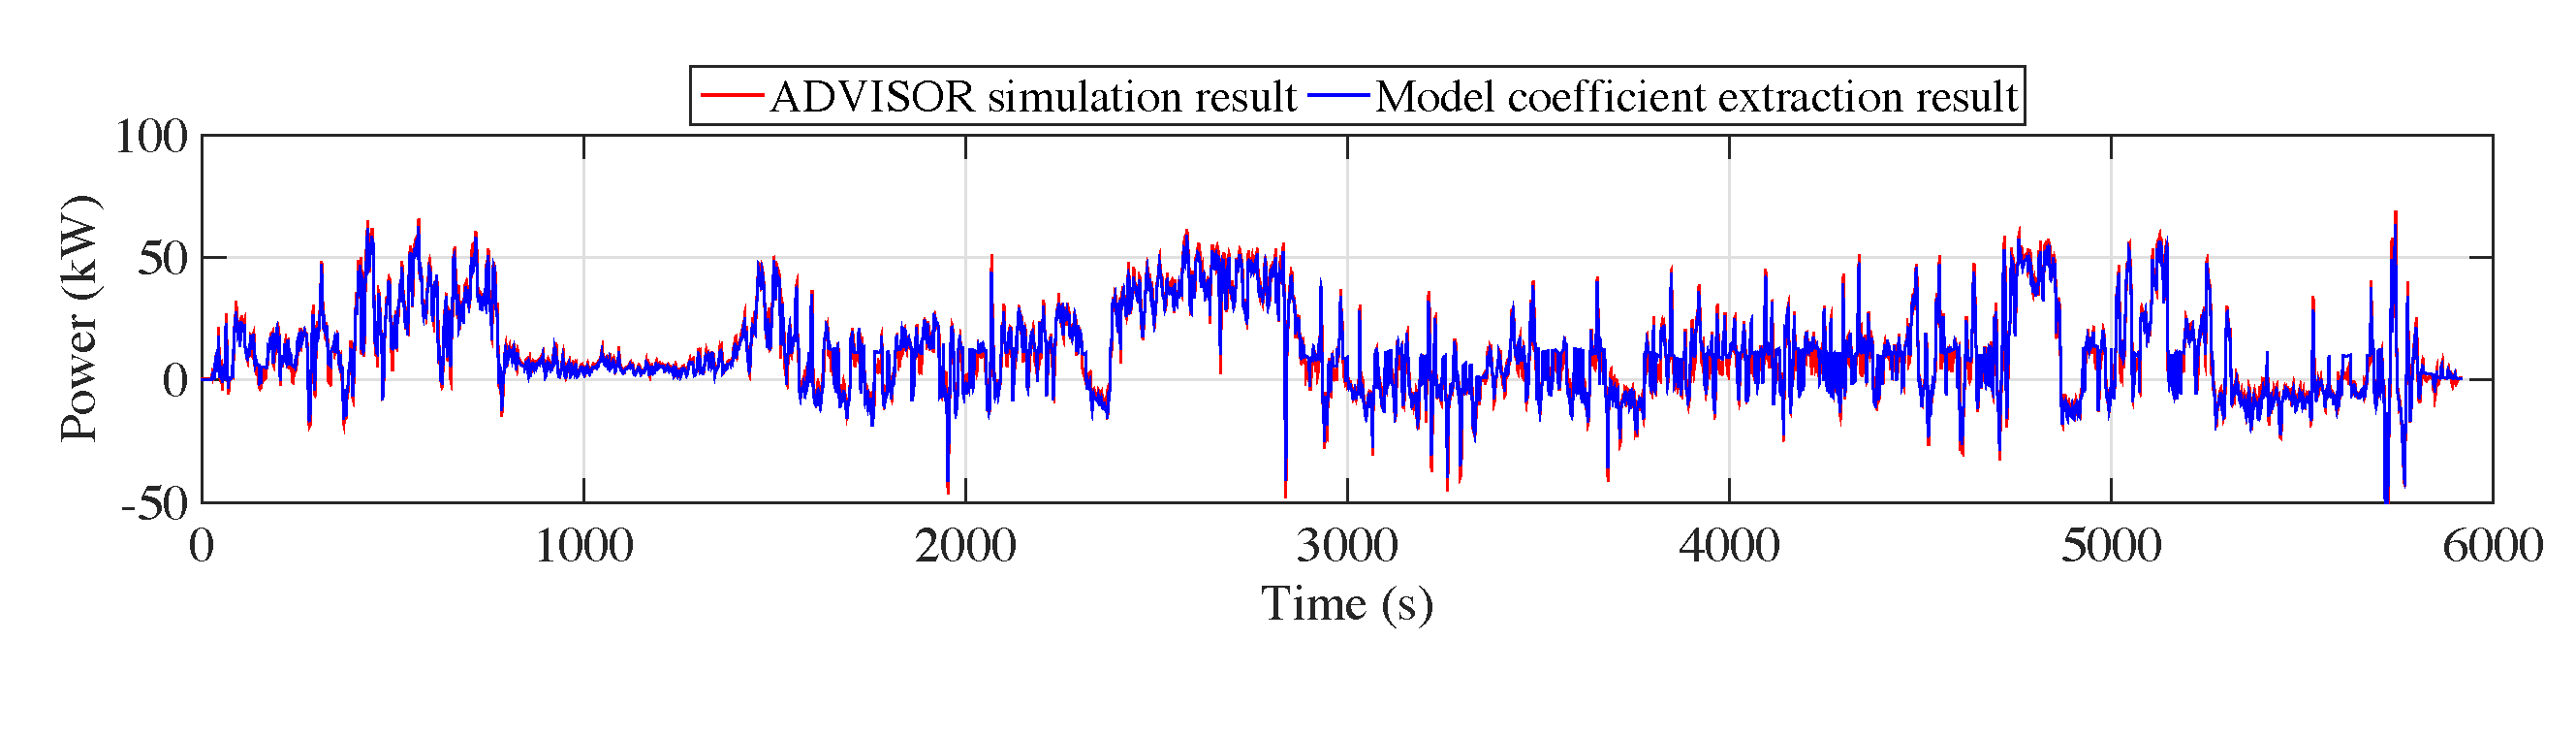
\includegraphics[width=1.0\hsize]{Figures/ADVISOR_model_validation_result.pdf}
\caption{Validation of the model coefficient extraction.}
\label{fig:ADVISOR_model_validation}
\end{figure*} 

ADVISOR is a vehicle simulator that takes into account various factors of vehicles including engines, electric traction motors, types of drivetrains, shape of chassis, etc.~\cite{Markel:JPS02}. ADVISOR is a fast simulator as it simulates a 700 second vehicle driving in one second. DP is commonly used to derive the energy-aware-velocity planning of vehicles~\cite{Lin:ICCA14,Dib:IVPPC11}. The DP optimization repeatedly computes the vehicle energy in each distance, velocity and acceleration step, and thus it is not proper to run ADVISOR in the inner loop of the DP optimization. For instance, it takes 15 minutes of computation to derive a 10 minute driving velocity planning profile with a 30-step velocity resolution. This is absolutely not acceptable for online recomputation that can be caused by unexpected interrupts while driving. So, instead of using ADVISOR for the speed optimization, we use ADVISOR for the model coefficient extraction. In other words, we use the same form of polynomial as~\eqref{eq:EV_specific_model} but derive the coefficients by running ADVISOR. 

\textcolor{red}{We can produce a new solution in a reasonable amount of time if an unexpected interrupt occurs. For example, if a vehicle accident occurs, a GPS navigator may perform rerouting to detour the accident area. The proposed velocity planning should be ``recomputed'' for the modified route. After detouring, the new route will be merged to the original route, and we can still reuse the previously computed  velocity planning for the rest of travel. While the proposed methods can perform such online ``recomputation,'' the previous method that uses ADVISOR in the inner loop can hardly meet such requirement.}

We choose Chevrolet Bolt (1,616 kg curb weight) for the target vehicle, but our method does not restrict a particular type of vehicles. \textcolor{red}{Chevrolet Bolt has been produced since November 2016. Total 26,000 units have been  delivered, and Bolt is positioned as the third best-selling EV in the United States.} The top speed of Chevrolet Bolt is a 150 km/h. It is capable of achieving a 6.5 second 0--100 km/h time with a 150 kW electric permanent magnet motor~\cite{GM_Bolt:official}. Chevrolet Bolt is equipped with a 350 V and 57.4 kWh Lithium-ion battery pack with 96-series and 3-parallel of 3.65 V cells~\cite{GM_Bolt:spec}. Chevrolet Bolt battery chemistry is Lithium Nickel Manganese Cobalt Oxide from LG. 

\begin{figure}   %Figure 1.
\centering
	\begin{subfigure}{0.4\textwidth}
	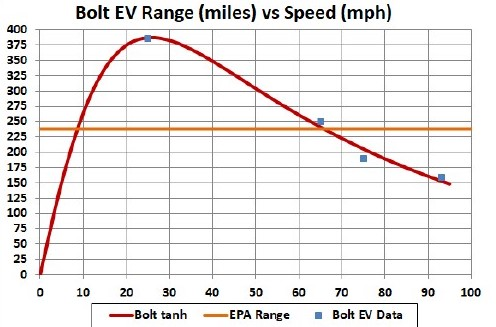
\includegraphics[width=\hsize]{Figures/Bolt_EV_range.jpg}
	\caption{}
	\label{fig:range_speed_exp}
	\end{subfigure}
~
	\begin{subfigure}{0.4\textwidth}
	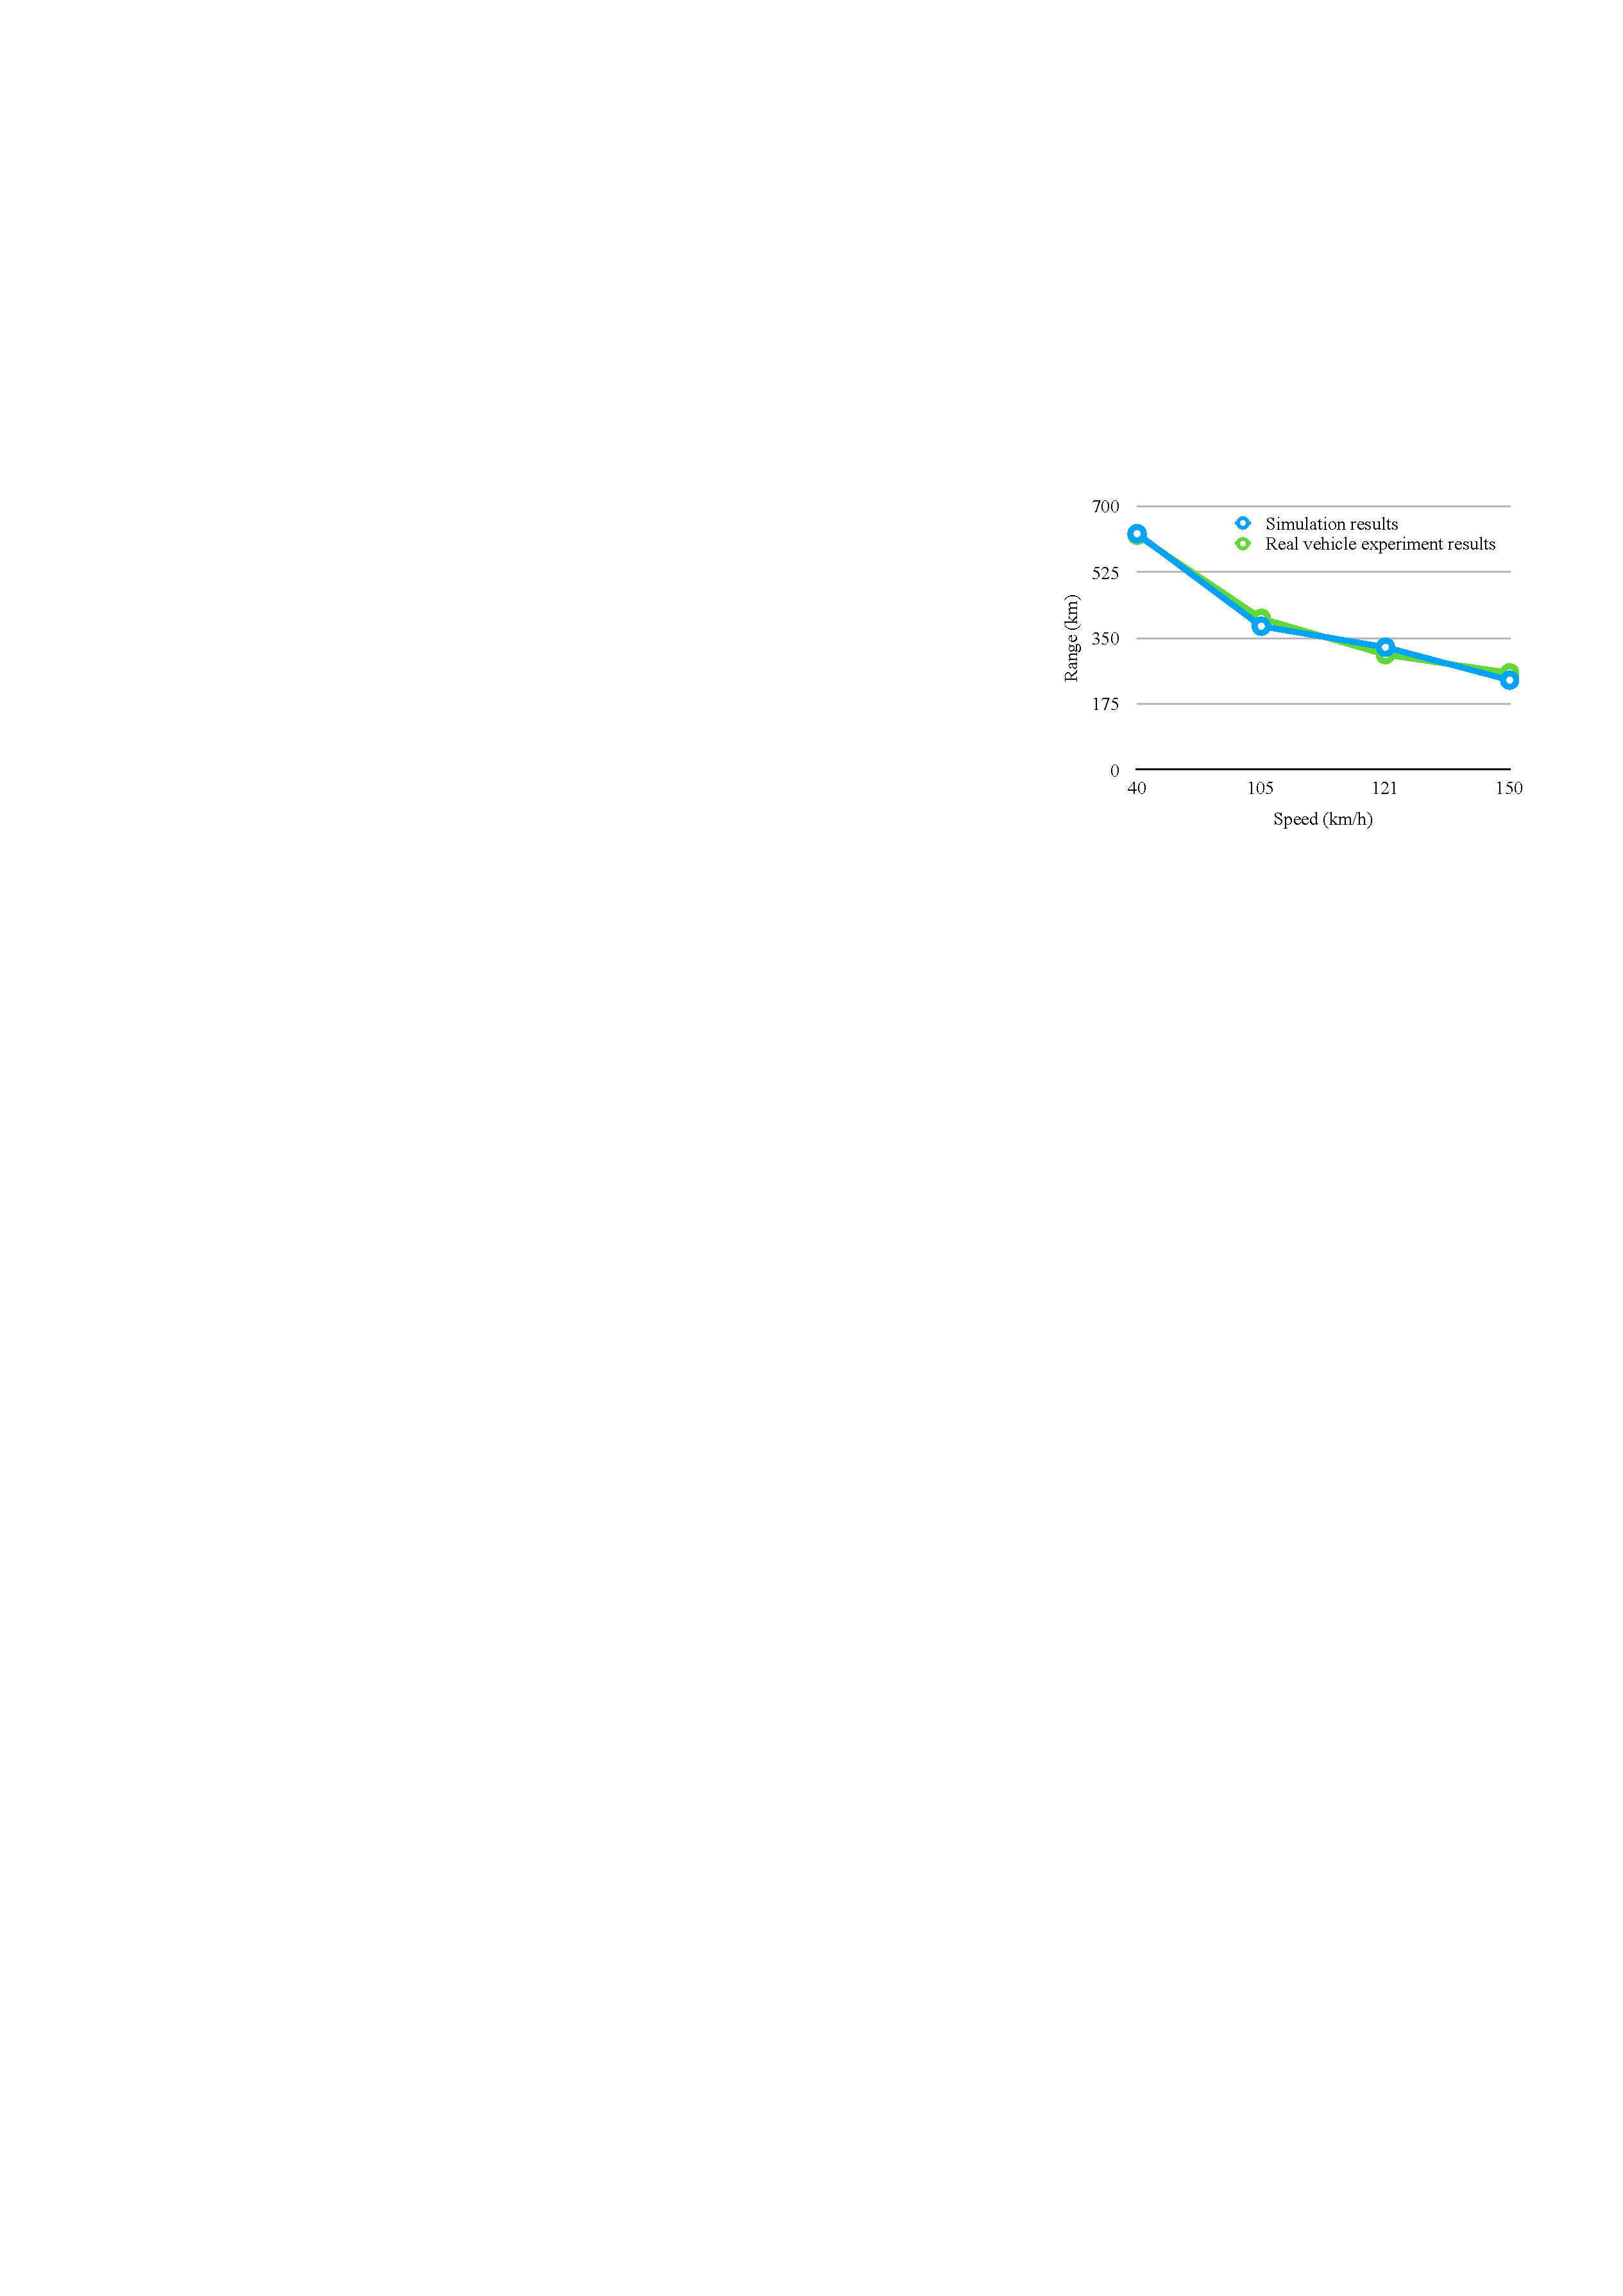
\includegraphics[width=\hsize]{Figures/Range-speed_validation.pdf}
	\caption{}
	\label{fig:range_speed_valid}
	\end{subfigure}
\caption{\textcolor{red}{(a) Range-speed experimental data for Chevrolet Bolt~\cite{GM_Bolt:range_speed} and (b) comparison with simulation results of the proposed EV power model.}}
\end{figure}

\textcolor{red}{We use ADVISOR to extract the model coefficients of new vehicles starting from known vehicle specifications such as the aerodynamic resistance, rolling resistance, curb weight, and so on. Such data is often published in the users' manual, website and so forth. We further use the vehicle performance data such as the top speed, maximum acceleration, and so on, which are also available on the manuals and website. We iteratively run ADVISOR and derive the model coefficients so that all the known values match among each other.}
The model coefficient extraction result shows as in Fig.~\ref{fig:ADVISOR_model_validation}. The normalized root-mean-square (RMS) deviation is 5.1\%. Table \ref{table:Coeff_Bolt} summarizes the model coefficients of (\ref{eq:EV_specific_model}) for Chevrolet Bolt. 

\textcolor{red}{We further evaluate the model accuracy with the range-speed real vehicle experiments as shown in Fig.~\ref{fig:range_speed_exp} to confirm the derived power models are close enough to the real vehicle measurement data~\cite{GM_Bolt:range25mph,GM_Bolt:range65mph,GM_Bolt:range75mph,GM_Bolt:range93mph,GM_Bolt:range_speed}. We  refine the coefficients until all the available data values match well. Finally, the derived EV power model well matches with the range-speed experimental data as shown in Fig.~\ref{fig:range_speed_valid} as well as the top speed and maximum acceleration setting the aerodynamic resistance, rolling resistance, curb weight, etc. with the known values. The errors of the range-speed simulation is merely 1.4\%, the time to approach 60 mph at departure is 7.8\%, and the top speed is 3.0\%, respectively.} 

\begin{table}
\caption{Model coefficients for Chevrolet Bolt.}
\label{table:Coeff_Bolt}
\centering
\begin{tabular}{|c|c|c|c|c|c|}  \hline
$\alpha$	&0.06		&$\beta$	&9.5549	&$\gamma$	&1.0013	\\ \hline
$\delta$	&0.00012 		&$C_0$	&1000 	&$C_1$		&10.588	\\ \hline
$C_2$	&8.11		&$C_3$	&0.00032	&$\epsilon$	&0.6633	\\ \hline
$\zeta$	&5813.6		\\ \cline{1-2}
\end{tabular}
\end{table}

%%%%%%%%%%%%%%%%%%%%%%%%%%%%%%%%%%%%%%%%%%
\subsection{Energy consumption comparison between ICEV and EV} \label{subsec:comparison}

We compare power consumption behavior of EV and ICEV in this section. As most previous fuel economy analysis work is done by energy (fuel) consumption, we compare energy consumption instead of power consumption for easy comparison. 

\begin{figure}	%Figure 3.
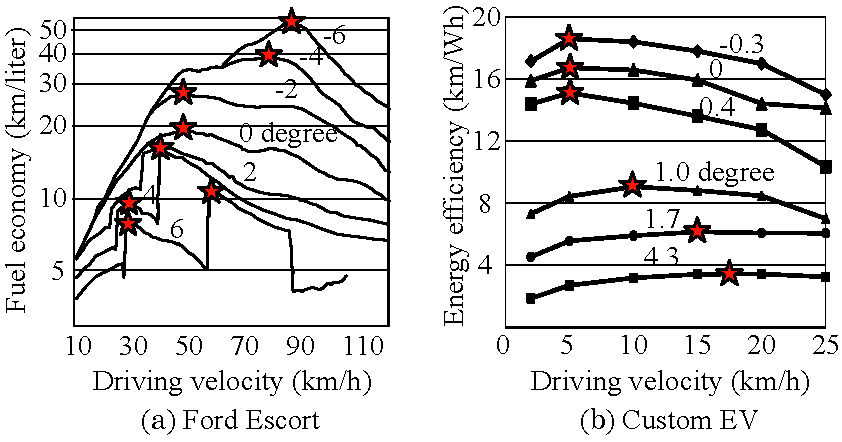
\includegraphics[width=1.0\hsize]{Figures/ICEV_EV_consumption.pdf}
\caption{(a) Fuel economy of a Ford Escort~\cite{Hooker:TR88} and (b) energy consumption of a custom EV~\cite{Chang:ICCAD14} on various road slopes and vehicle velocities.}
\label{fig:ICEV_EV_consumption}
\end{figure} 

Fig.~\ref{fig:ICEV_EV_consumption}(a) shows the fuel economy (range with a liter of fuel energy) versus ICEV velocity on various road slopes~\cite{Hooker:TR88}. Red stars denote  the minimum-energy velocity by the average road slope. The minimum-energy velocity is reduced as the road slope increases. For example, the vehicle has the highest fuel economy at 90 km/h on  a $-6$ degree road slope and 40 km/h on a 2 degree road slope.  Fuel economy on a downhill (negative road slope) is not meaningful due to  \textit{fuel cut} of modern ICEVs. Compared with the flat road (zero degree), we see the fuel economy drops if the road slope is steeper than 2 degree due to downshift of the transmission. 

Fig.~\ref{fig:ICEV_EV_consumption} demonstrates a very interesting EV-specific energy behavior such that the least-energy velocity increases as the road slope increases. Such energy behavior is completely opposite to that of ICEV. 
%
The efficiency maps of an  engine and an electric motor (Fig.~\ref{fig:efficiency_map}) show that the motor exhibits  the maximum torque over the wide range of RPM while the engine exhibits the maximum fuel efficiency only at near 2,000 RPM. Therefore, an engine should be incorporated with a transmission that makes it possible to run the engine at close to the most efficient region, independent to the vehicle velocity. The required engine torque multiplied by the gear ratio (determined by the transmission shift position) also changes by the vehicle gradient resistance (road slope.) The optimal  transmission shift position and the least-energy velocity are thus determined by the road slope.

On the other hand, a fixed ratio gearbox is generally sufficient for EV since electric motors obtain the maximum torque over the wide range of RPM. The least-energy velocity is solely determined by the motor efficiency, which is a function of the torque and RPM. 
%
\begin{align}
E_{EV^*} 	&= \int_{T_{drive}} P_{EV^*}(v_{const})~dt \nonumber\\
		&= \frac{P_{trac}}{\eta_{EV}(T, \omega)} \int_{T_{drive}} dt  \nonumber\\
		&= \frac{F_{trac} \times v_{const}}{\eta_{EV}(T, \omega)} T_{drive}
		= \frac{F_{trac} \times D_{drive}}{\eta_{EV}(T, \omega)} \nonumber
\end{align}
where $T_{drive}$, $V_{const}$ and $D_{drive}$ denote the driving time, constant velocity and driving distance, respectively. Energy consumption, $E_{EV}$, with a constant velocity on a given road slope is sorely determined by the motor efficiency, $\eta_{EV}$. 

As the road slope becomes higher, the motor RPM would better be increased to achieve a higher motor efficiency according to the motor efficiency map in Fig.~\ref{fig:efficiency_map}(b). The least-energy velocity of EV increases as the RPM increases because of the fixed single ratio gearbox. It is not possible to derive the least-energy velocity for EVs by applying that for ICEVs because of such discrepancies in the powertrains.

\begin{figure}	%Figure 4.
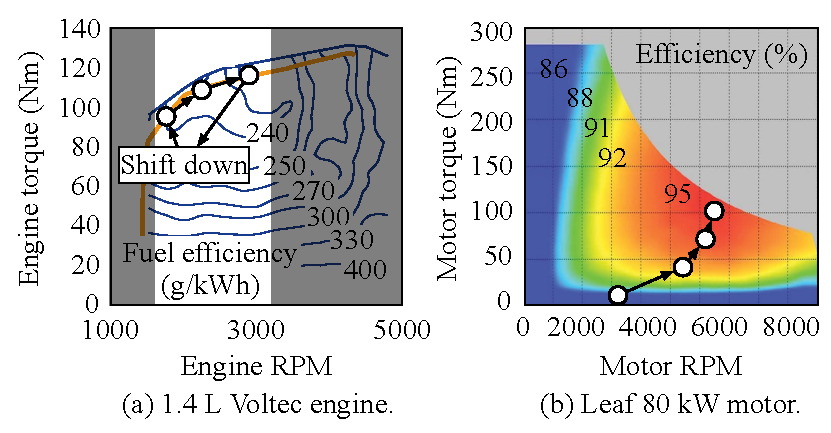
\includegraphics[width=1.0\hsize]{Figures/efficiency_maps.pdf}
\caption{Efficiency maps of (a) the GM 1.4 liter Voltec engine and (b) the Nissan Leaf 80 kW electric motor.}
\label{fig:efficiency_map}
\end{figure} 

%%%%%%%%%%%%%%%%%%%%%%%%%%%%%%%%%%%%%%%%%%
\section{Framework for Energy-Aware-Velocity Planning} \label{sec:framework}
%%%%%%%%%%%%%%%%%%%%%%%%%%%%%%%%%%%%%%%%%%

%%%%%%%%%%%%%%%%%%%%%%%%%%%%%%%%%%%%%%%%%%
\subsection{The least-energy-constant-velocity driving} \label{subsec:constant drive}

\begin{figure} %Figure 5.
\centering
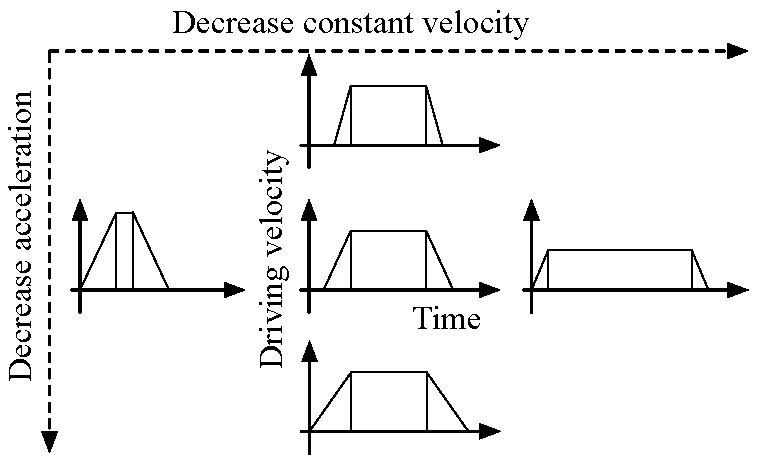
\includegraphics[width=0.85\hsize]{Figures/const_vel_drive_problem.pdf}
\caption{Various constant velocity and acceleration cases for the same distance.}
\label{fig:const_vel_drive_problem}
\end{figure} 

A constant-velocity driving is not always impractical and actually  useful to ensure a steady traffic flow and safety. Drivers often drive their vehicles up to the speed limit or slightly over the speed limit following the flow mainly aiming at the shortest possible driving time. However, when it comes to the energy-aware-velocity planning, a constant-velocity driving should be set to the least-energy velocity. 

We demonstrate how the cruising velocity, acceleration and deceleration affect EV energy consumption. We perform a design space exploration (DSE) for all feasible vehicle velocities and the acceleration pairs. We obtain the minimum-energy velocity and the initial and final acceleration for a given driving distance  as shown in Fig.~\ref{fig:const_vel_drive_problem}. The results of DSE on a flat road (0 degree road slope) and a 4 degree road slope are shown in Fig.~\ref{fig:DSE}(a) and \ref{fig:DSE}(b), respectively. The point at the minimum energy consumption per distance (Wh/km) represents the least-energy-constant-velocity driving. Surprisingly, the same distance driving requires significantly different amount of energy by the cruising velocity and acceleration as shown in Fig.~\ref{fig:const_vel_drive_problem}. The energy consumption by the cruising velocity and acceleration pairs also completely changes by the road slopes. These examples indeed show a great potential to save energy consumption of EV with the proposed energy-aware-velocity planning.

\begin{figure} %Figure 6
\centering
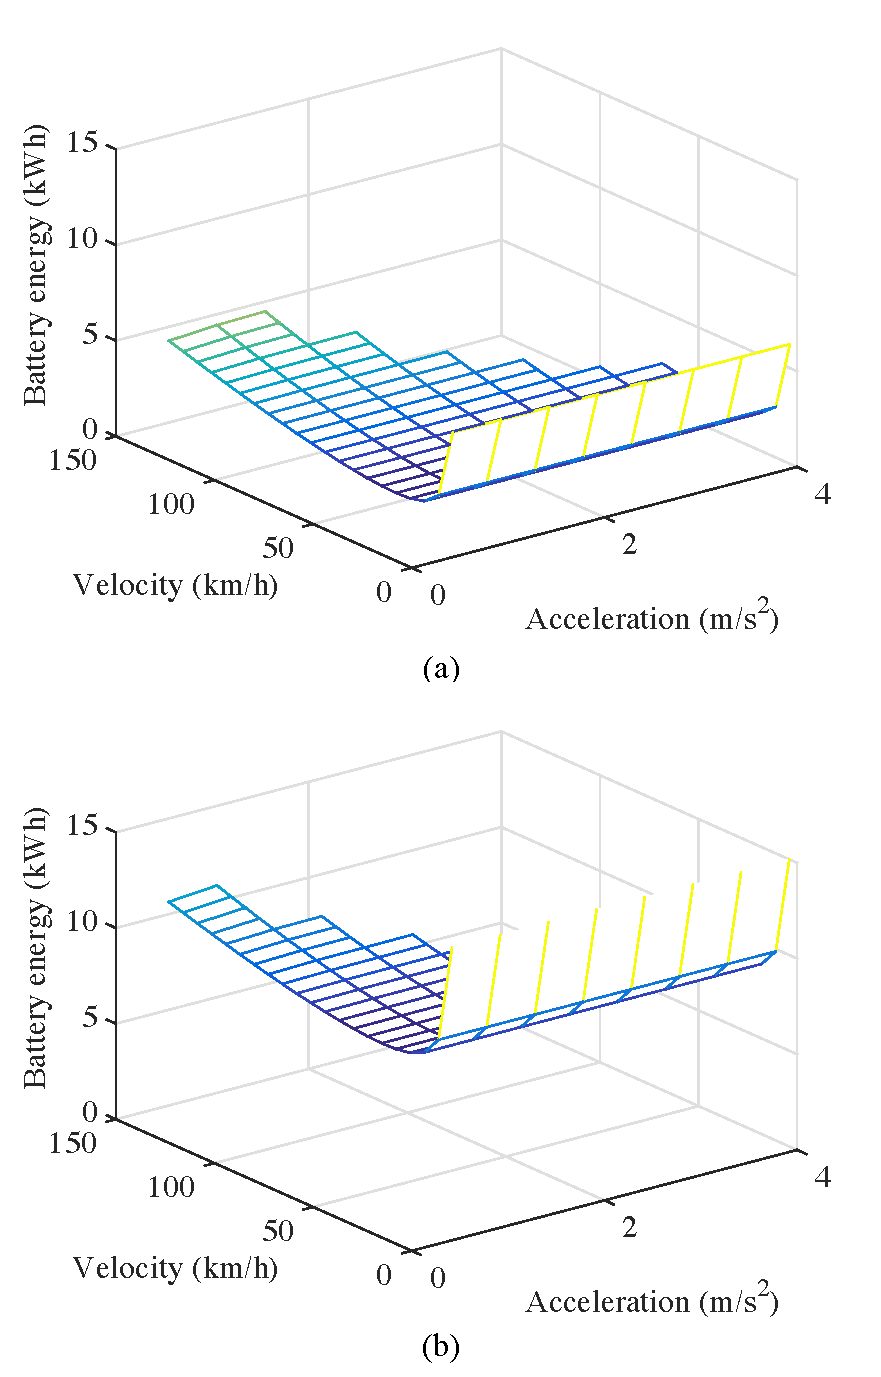
\includegraphics[width=0.85\hsize]{Figures/Design_space_exploration.pdf}
\caption{DSE of  the constant-velocity driving on (a) a 0 road slope and (b) a 4 road slope.}
\label{fig:DSE}
\end{figure} 

%%%%%%%%%%%%%%%%%%%%%%%%%%%%%%%%%%%%%%%%%%
\subsection{The minimum-energy-velocity planning} \label{subsec:variable drive}

\begin{figure} [h]%Figure 7
\center
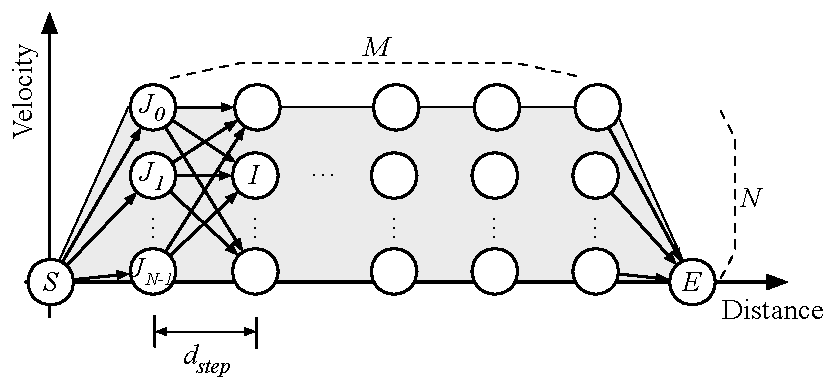
\includegraphics[width=0.85\hsize]{Figures/Opt_drive_problem.pdf}
\caption{Problem formulation to explore the minimum-energy-velocity planning.}
\label{fig:Opt_drive_problem}
\end{figure}

This subsection introduces a generalized minimum-energy-velocity planning for EV  on a road with variable slopes. We construct a DP to find the minimum-energy-velocity over distance. The DP obtains a set of the minimum-energy-velocity values for every distance step. In Fig.~\ref{fig:Opt_drive_problem}, the X-axis and Y-axes denote the driving distance from the starting point and the driving velocity, respectively. Each node indicates the driving velocity at a given distance, and an edge between two nodes implies acceleration or deceleration during the distance step ($d_{step}$.) The maximum velocity is $v_{max}$, and the velocity step between two nodes at the same distance is $v_{step}$. The number of the nodes in each distance step is $N = v_{max} / v_{step}$, and the number of edges for the distance step is $N^2$. One node has $N$ edges going to the next distance, and a node receives $N$ edges. For example, a set of previous nodes, $J_0, J_1, \cdots, J_{N-1}$, goes to the next distance node (Node $I$.) As the total number of steps to the endpoint is $M = (\rm driving~distance) / d_{step}$, total number of nodes and edges are $MN$ and $MN^2$, respectively. There are only two nodes indicating 0 $m/s$ at the starting point (Node $S$) and endpoint (Node $E$.) A solution of the problem is a sequence of a node selection every distance step from Node $S$ to Node $E$. The objective and the constraints are defined as
%
\begin{align} %Equation 6
Min ~& \sum_{d=1}^{M}\sum_{v=1}^{N}\{\Delta t \frac{x(d,v)P_{d,v} + x(d-1,v)P_{d-1,v}}{2}\} \label{eq:objective}\\
Subject~to ~& \sum_{v=1}^{N}x(d,v) = 1~~where~~x(d,v) = \{0, 1\} ~~~\forall d, v \nonumber
\end{align}
%
where $\Delta t$ is a time to pass the distance step with a given velocity $v$, $d$ is the distance from the starting point and $P_{d,v}$ is the power consumption for a node with $d$ and $v$. $\Delta t$ varies by the driving velocity and acceleration. We set $x(d,v)=1$ once we accept the node at the distance $d$ and the velocity $v$.


\textcolor{red}{\subsection{Real Road Benchmarking Set}} \label{subsec:benchmark}

\textcolor{red}{We implement six real routes from various locations in California. The first three routes consist of road segments in cities. Jones Street in San Francisco and Hoover Street in Los Angeles are two representative city landscapes such as hills and flat roads, and Cliff Drive in Santa Barbara is a mixture of those. The second two routes are road segments in mountain areas: Serrano Avenue in Anaheim Hills and Otay Lakes Road in San Ysidro Mountain in California. The last route is Junipero Serra Boulevard connecting San Fransisco and San Jose. The details of route data is summarized in Table \ref{table:road_bench}, and Fig. \ref{fig:bench_altitude}, which visualize the altitudes of the benchmarking routes.}

\begin{table} 
\caption{\textcolor{red}{Real road benchmarks.}}
\centering
\label{table:road_bench}
\begin{tabular}{|c|c|c|c|c|c|c|}  \hline
\multirow{2}{*}{Roads} 
				&Dist.		&\multicolumn{5}{|c|}{Road slope (\%)}  \\ \cline{3-7}
				&(m)		 	&Max.		&Min. 	&Mean		&RMS 	&Std.	\\ \hline
Jones St. 	&1257		&29.22		&-15.12	&4.97 		&12.31 	&11.27	\\ \hline
Hoover St. 	&1365		&8.45		&-7.44	&0.44		&1.08 	&0.99	\\ \hline
Cliff Dr. 	&1435		&4.77		&-2.75	&0.58		&1.77 	&1.67	\\ \hline
Serrano Ave.		&1797		&16.63		&-10.56	&1.14 		&4.10 	&3.94	\\ \hline
Otay Lakes Rd.		&1623		&6.80		&1.12	&3.24		&3.52 	&1.38	\\ \hline
Junipero Serra Blvd.	&1500		&7.46		&-5.48	&0.40		&2.72 	&2.70	\\ \hline
\end{tabular}
\end{table}


\begin{figure}	 %Figure 8.
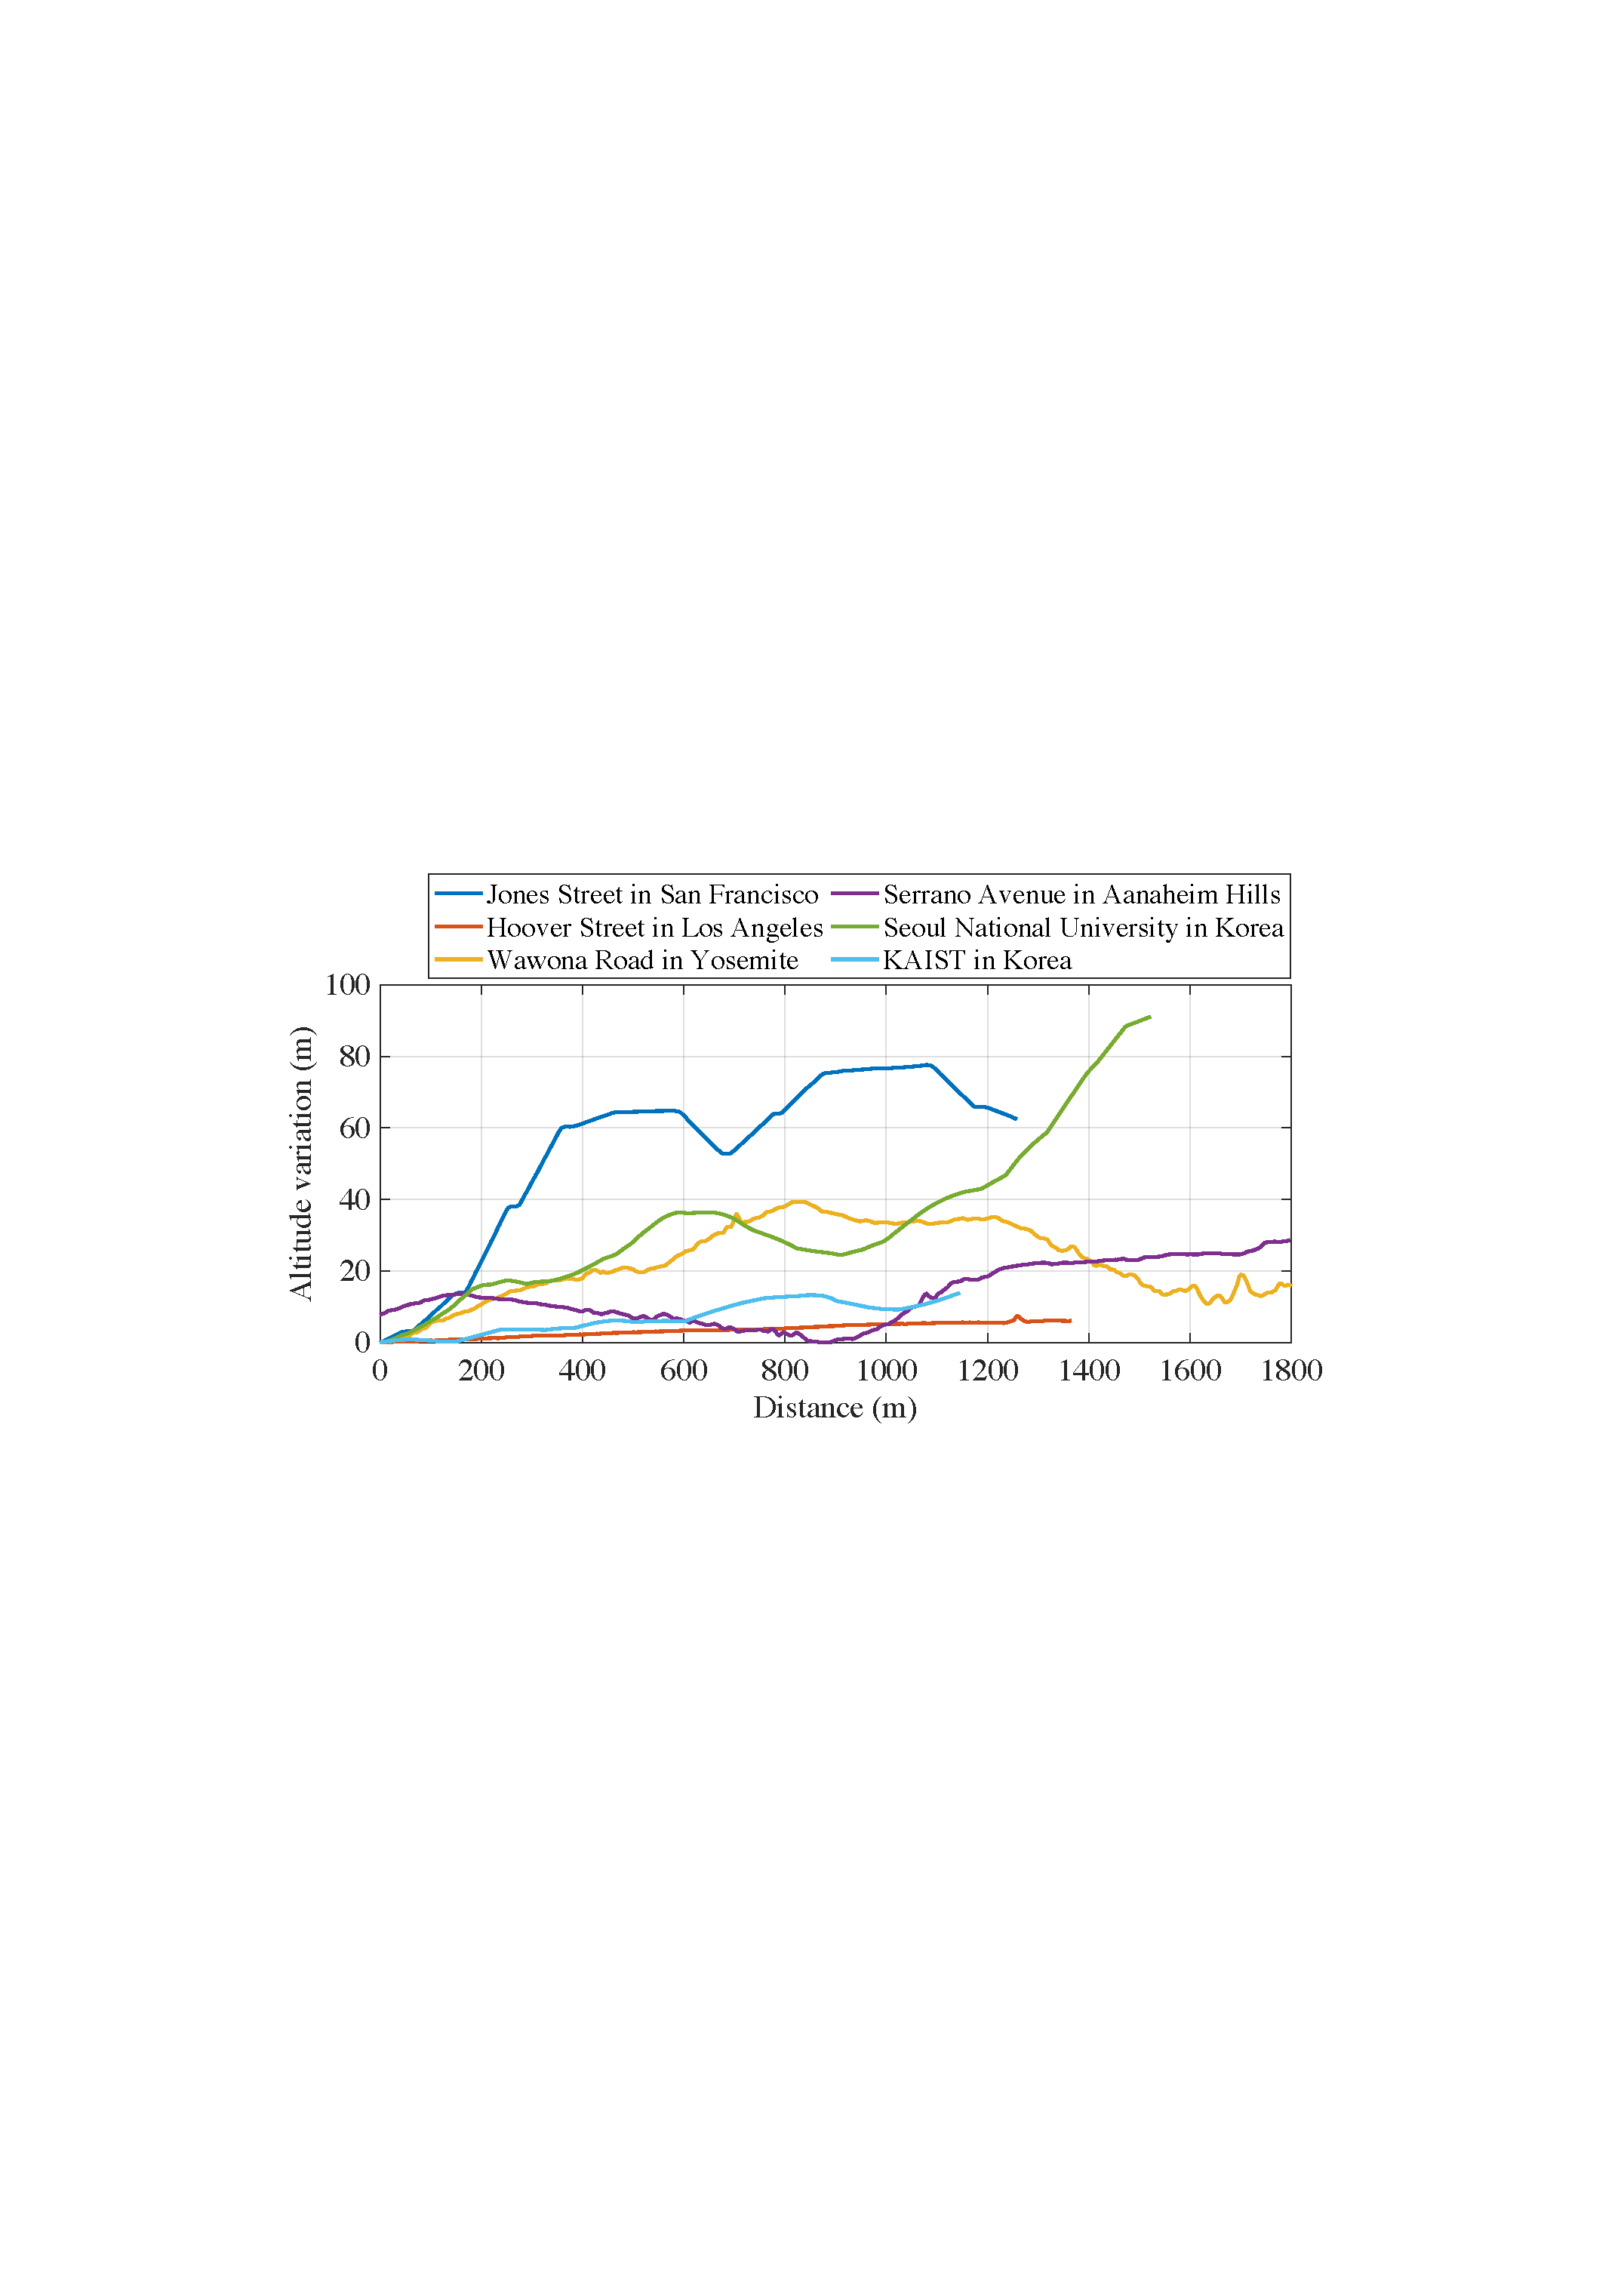
\includegraphics[width=1.0\hsize]{Figures/Benchmark_altitude.pdf}
\caption{\textcolor{red}{Benchmark altitude.}}
\label{fig:bench_altitude}
\end{figure} 


\textcolor{red}{\subsection{Consideration of both energy and time}} \label{subsec:energy_time}


The minimum-delay-constant velocity is determined by the speed limit of the driving route. The minimum-delay-constant velocity is 65 km/h, which is the maximum speed of the benchmark route.
The minimum-energy-velocity planning guides to speed up the vehicle before entering an uphill. As a result, the EV consumes less energy consumption compared with the least-energy-constant-velocity driving at the top elevation. The minimum-energy-velocity planning also reclaims more energy from the regenerative braking when the EV finishes the drive. The extended range by the minimum-energy-velocity planning is 17.2\% with the same battery capacity.

\begin{figure}   %Figure 9.
\centering
	\begin{subfigure}{0.4\textwidth}
	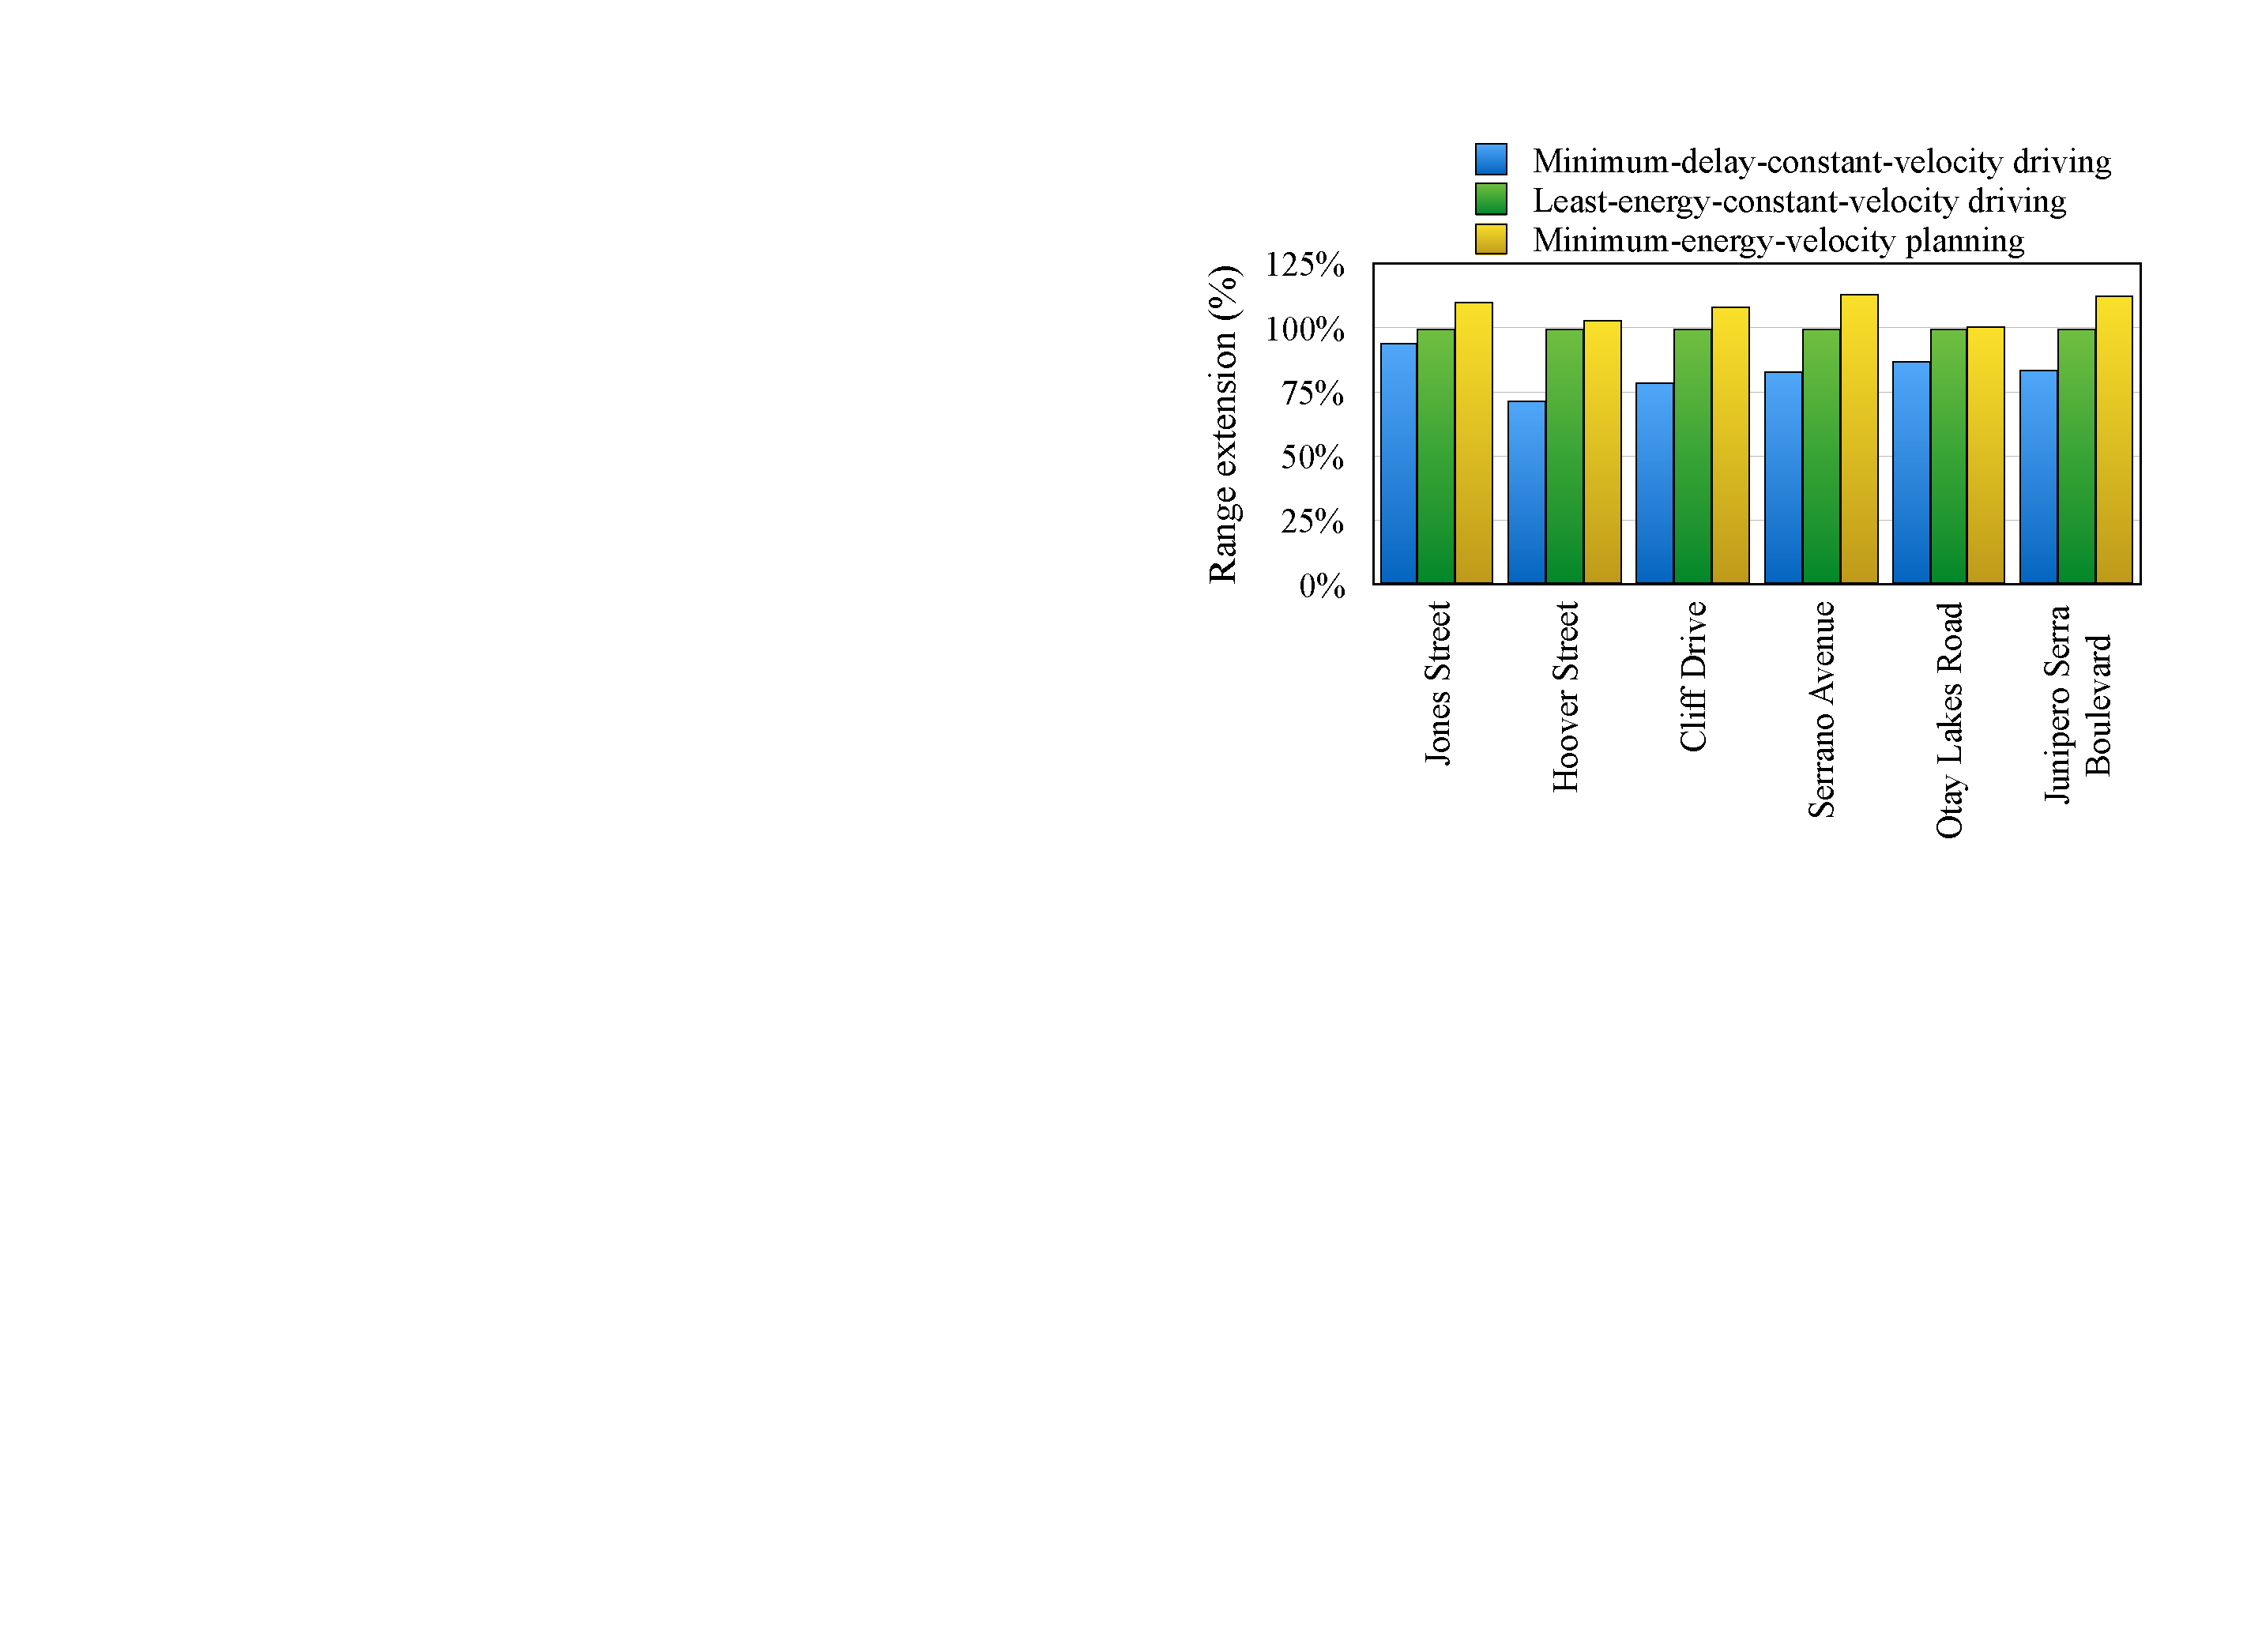
\includegraphics[width=\hsize]{Figures/range_comp_bar.pdf}
	\caption{}
	\label{fig:range_comp}
	\end{subfigure}
~
	\begin{subfigure}{0.4\textwidth}
	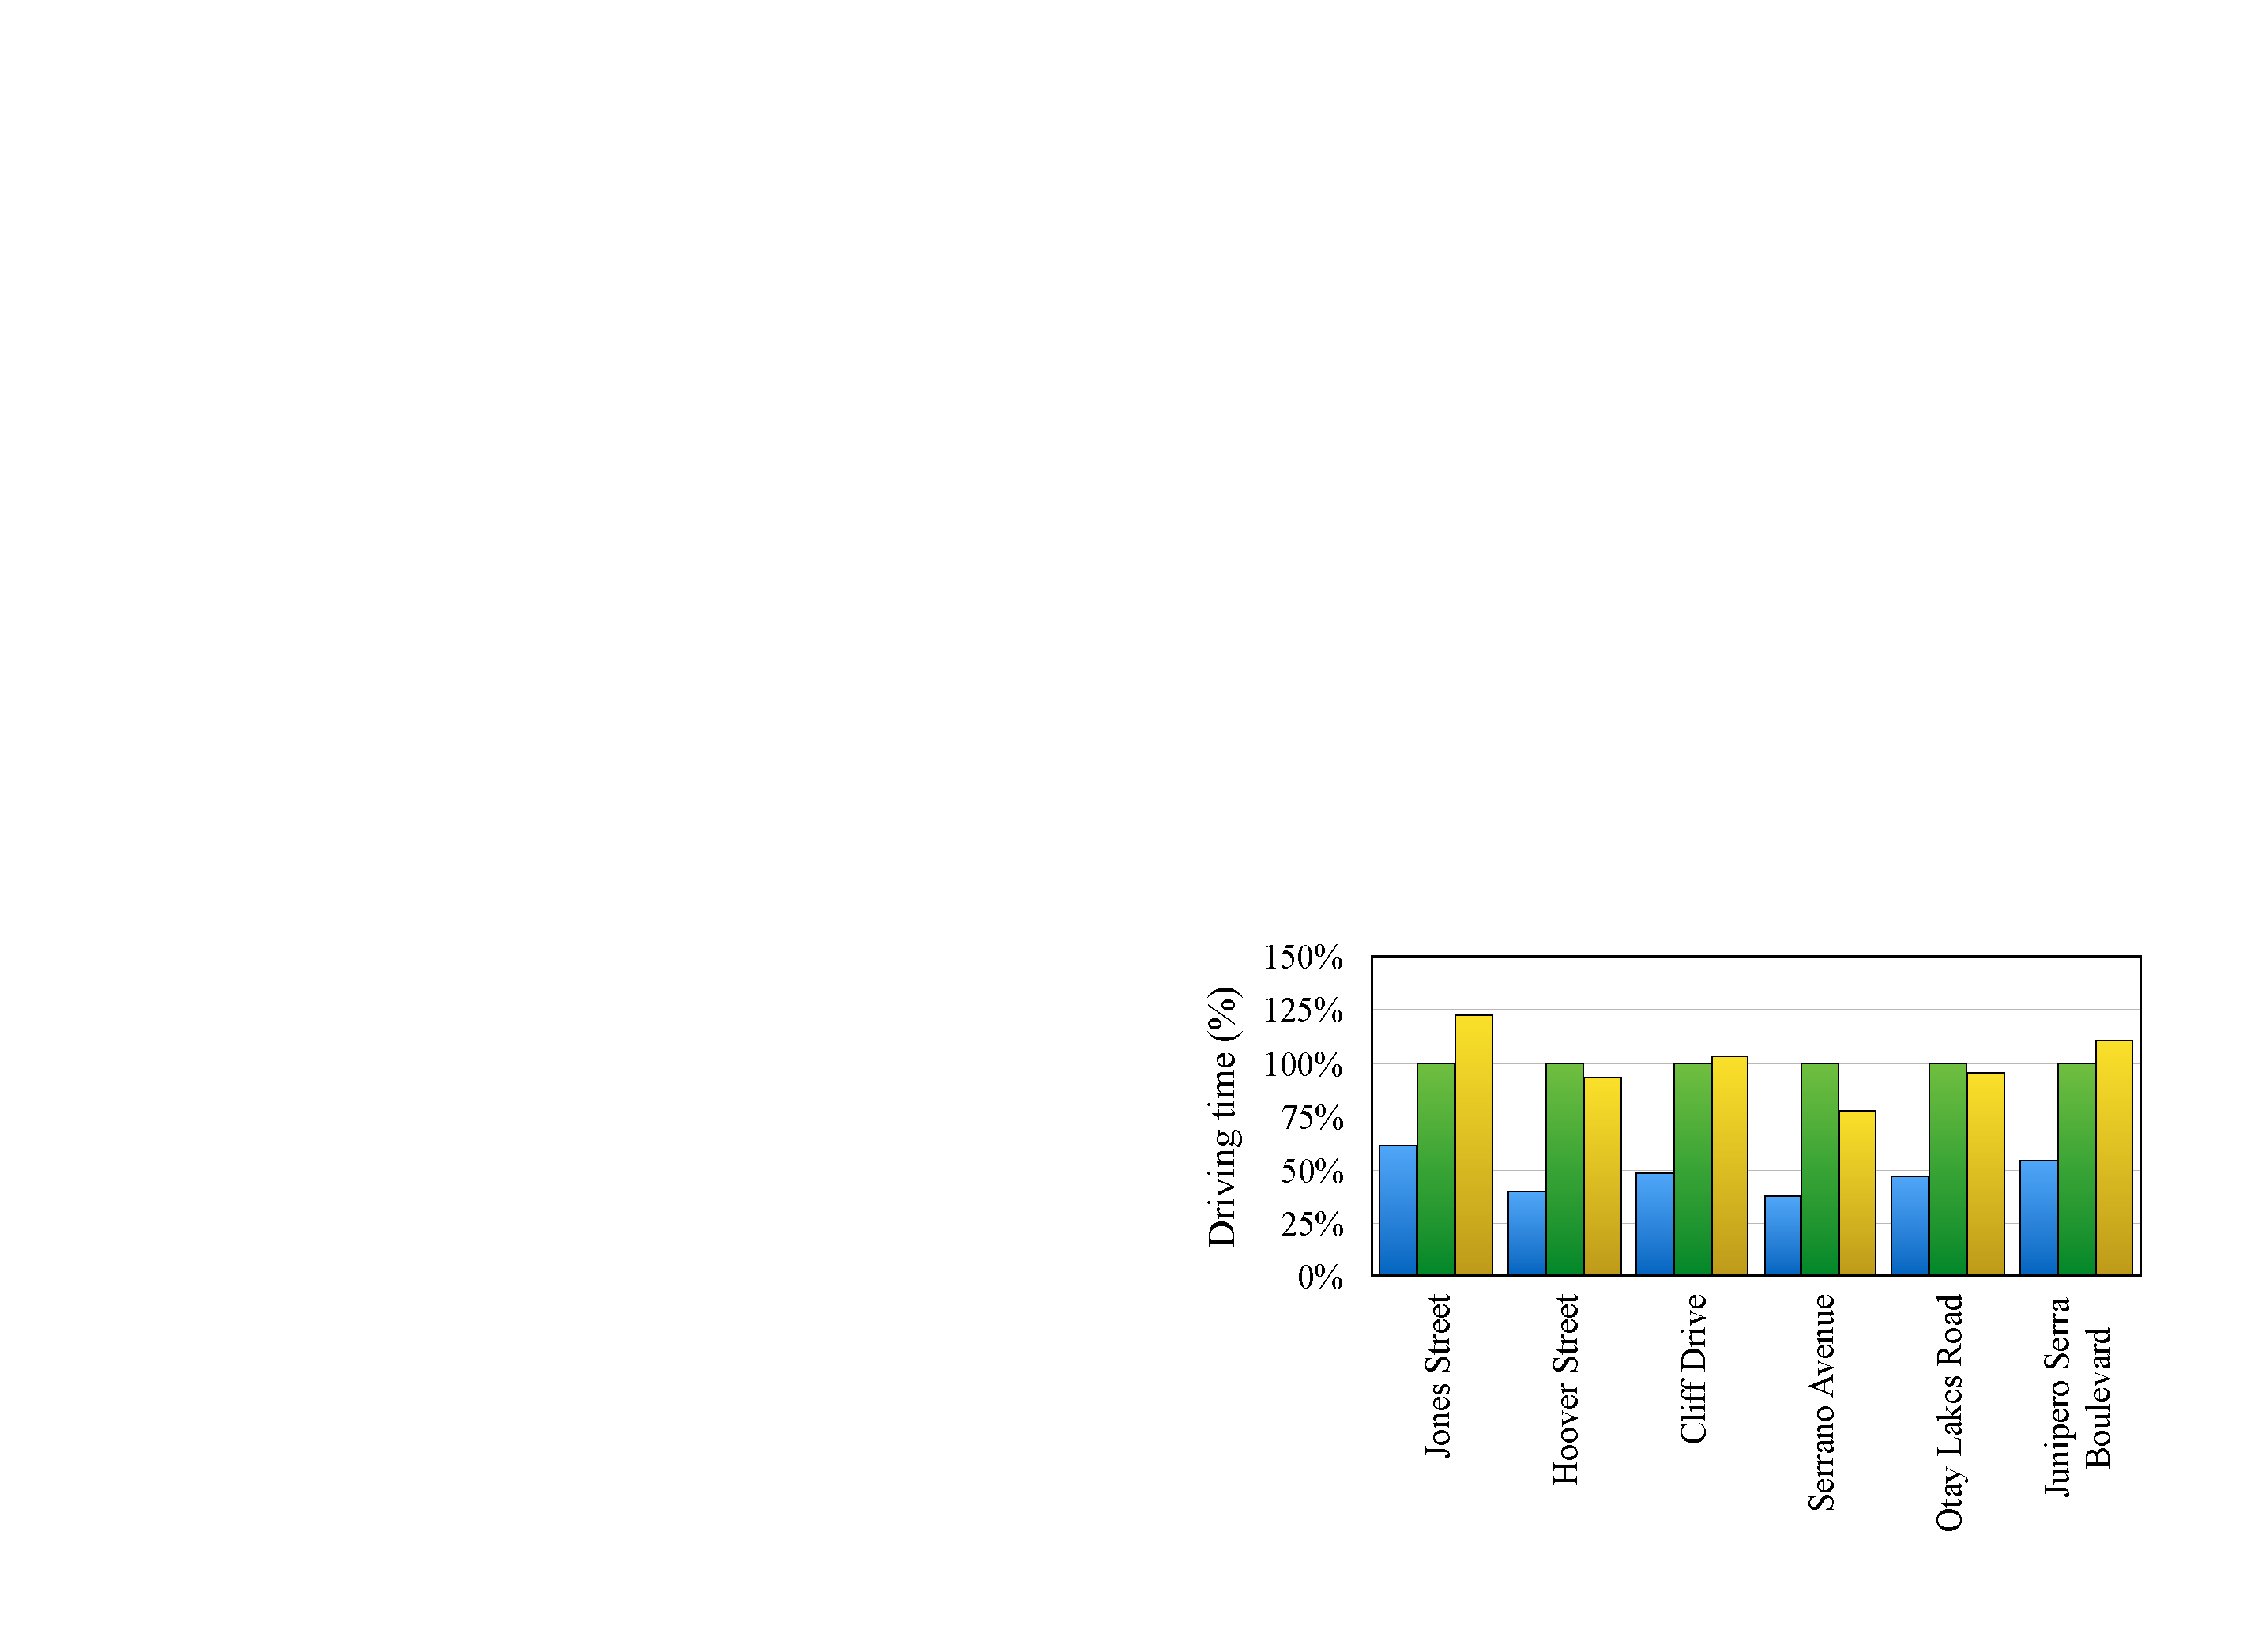
\includegraphics[width=\hsize]{Figures/driving_time_comp_bar.pdf}
	\caption{}
	\label{fig:driving_time_comp}
	\end{subfigure}
\caption{\textcolor{red}{(a) Range extension and (b) related driving time by the minimum-energy-velocity planning.}}
\label{fig:min_energy_planning_comp}
\end{figure}

\begin{figure}[h]
\centering
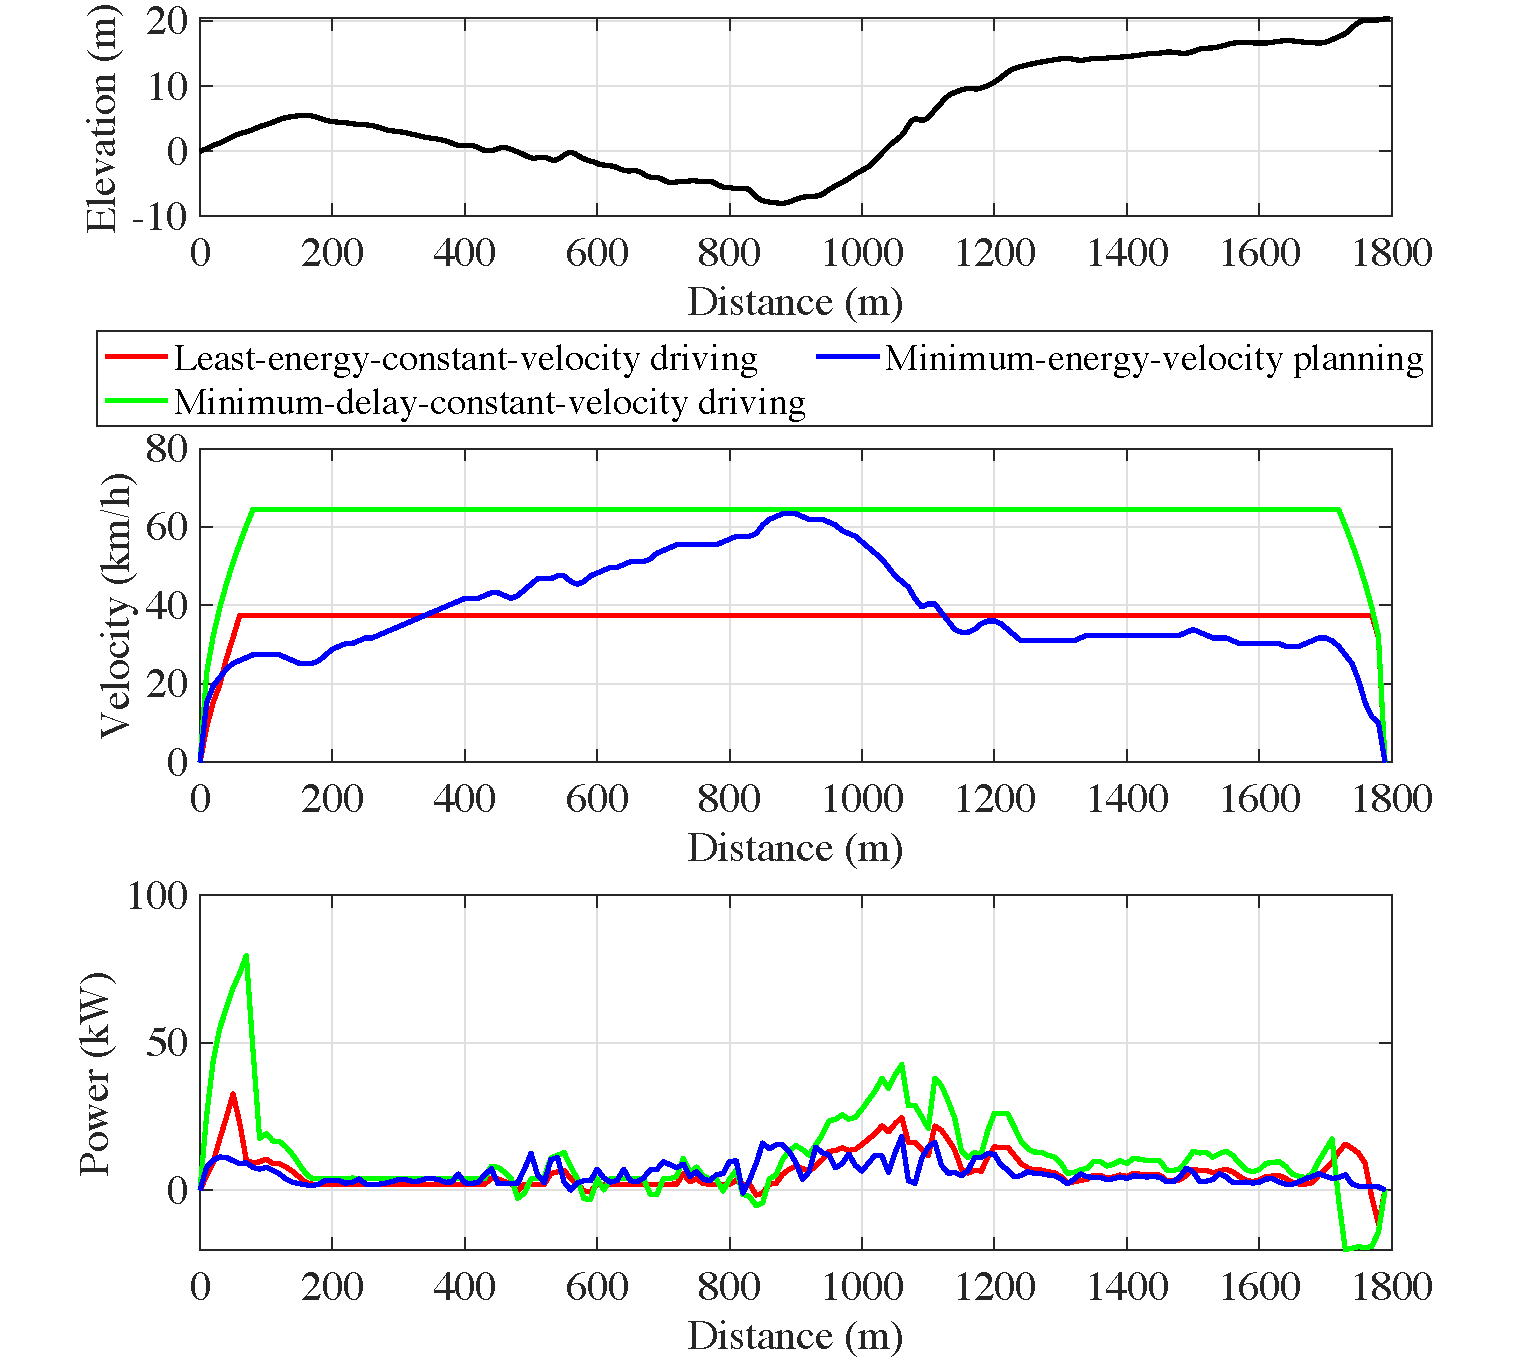
\includegraphics[width=\hsize]{Figures/energy_driving_profile_best.pdf}
\caption{Results of the minimum-energy-velocity planning.}
\label{fig:no_deadline_trace}
\end{figure} 

Fig.~\ref{fig:min_energy_planning_comp} shows the range extension and related driving time by the proposed minimum-energy-velocity planning on the benchmarking routes. Y-axis denotes the range extension compared with the least-energy-constant-velocity driving. Blue-colored bars indicate the minimum-delay-constant-velocity driving, and green-colored bars indicate the least-energy-constant-velocity driving, which are the baseline. Yellow-colored bars indicate the minimum-energy-velocity planning.

The range extension by the minimum-energy-velocity planning is from 2.8\% up to 17.2\% compared with the least-energy-constant-velocity driving. 
The minimum-energy-velocity planning extends the range on the two routes (Serrano Avenue and Junipero Serra Boulevard.) Unlike other routes, these two routes have relatively large RMS (root mean square) values and small mean values. This means that these routes include both uphill and downhill, and there are many chance to save energy consumption when entering uphill and downhill. 
On the other hands, routes having small standard deviations show less range extension compared with the least-energy-constant-velocity driving because constant-velocity driving is close to the optimal for the monotonous road slope.

\textcolor{red}{Even though the minimum-energy-velocity planning exhibits a significant amount of range extension compared with the minimum-delay-constant-velocity planning, the resultant driving time become too long, i.e., the EV drives too slow. Too slow driving may bother other traffic as well as making the driving too time consuming. So, we assume that the EV should not drive too slow to avoid bothering traffic with the minimum speed of a 25 km/h. %Even with the minimum speed constraint as lower than 25 km/h, we exhibit the same amount of gains with the proposed methods.}
%
We enforce the minimum acceleration not lower than 0.4 $m/s^2$ when the EV starts from a stop sign or a traffic light until the velocity reaches to 25 km/h not too bother traffic flow. If the EV accelerates at a 0.4 $m/s^2$, it would take 15 seconds to reach a 25 km/h speed. 
%
The maximum acceleration is limited by the motor torque: a 4.7 $m/s^2$ on a flat road.  However, such a fast acceleration negatively affects to the  power consumption as well as passenger comfortness. We limit the maximum acceleration to 1.7 $m/s^2$ as shown in Fig.~\ref{fig:histogram}(b), which is the same as the maximum acceleration of compact cars designed to be used primarily used in urban areas (15 seconds of 0 to 100 km/h time).}\\


\textcolor{red}{We compare the simulation results among the least-energy-constant-velocity driving, the minimum-delay-constant-velocity driving and the minimum-energy-velocity planning. Fig.~\ref{fig:no_deadline_trace} shows altitude of Serrano Avenue, the velocity planning results and power consumptions by each method, respectively. 
We perform a design space exploration (DSE) for all feasible vehicle velocities and the acceleration pairs to derive the least-energy-constant-velocity driving. The point at the minimum energy consumption per distance (Wh/km) represents the least-energy-constant-velocity driving. The least-energy-constant velocity is 37 km/h in this example.}

The minimum-energy-velocity planning solely considers the energy consumption, which may make the vehicle velocity impractically slower in many cases. 
%This phenomenon becomes more distinct when the road is flat. 
In fact, most production EVs exhibits the longest range when the vehicle velocity is around 30 km/h on a flat road \textcolor{red}{as shown in Fig.~\ref{fig:range_speed_exp}.} Nevertheless, energy for cruising is much lower than energy for acceleration and diving uphills while the cruising velocity significantly affects the driving time. \textcolor{red}{For example, the minimum-delay-constant-velocity driving reduces driving time considerably by sacrificing range for routes having small standard deviation (Hoover Street, Cliff Drive and Otray Lakes Road).}





\subsection{$EDP$-aware-velocity planning} \label{sec:ed_consideration}

% Energy-delay curve 
%This subsection introduces energy-delay characteristics of EV to combat the energy consumption and driving time tradeoff more systematically. 
%The energy-delay curves show the merit of the proposed velocity planning compared with the least-energy-constant-velocity driving with a deadline. 
%We plot the relationship between driving energy and driving time with deadline constraints in Fig.~\ref{fig:energy_delay_curve}. X-axis and y-axis denote the EV driving time and energy under given deadlines, respectively. The energy-delay plot is useful to figure out the Pareto optimal velocity profiles. The energy-delay curves of the minimum-energy-velocity planning are located under the least-energy-constant-velocity driving curves, which implies that the minimum-energy-velocity planning is better than that of the least-energy-constant-velocity driving in terms of energy consumption under the same deadline. The same is true for the driving time under the same energy budget.

It is not an easy problem to consider both driving energy and driving time. Previous work attempts to consider driving time to make a single optimization metric with energy and time as a weighted sum of them \cite{Lin:ICCA14,Mensing:TR13,Dib:IVPPC11}. This method is to deal with tradeoff between the energy and time, but it is not intuitive to determine the weight factors because the weight factors cannot explicitly control the tradeoff.
The other method used in the previous work is Genetic Algorithm (GA.) GA solves multi-objective optimization problems, and therefore, it provides a good quality solution to take both energy and time into account~\cite{Dovgana:ASC14,Grossard:ISIE12}. However, GA is not for online computation, which is hard to apply for the energy-aware-velocity planning that requires potential frequent online recomputation due to unexpected interrupts. 

In this paper, we propose to use energy-delay product ($EDP$), energy-square-delay product ($E^2DP$), or energy-cubic-delay product ($E^3DP$) so that a single metric can consider both energy and driving time while we are able to explicitly manipulate $EDP$.

DP is a method for solving a complex problem by breaking it down into a collection of simpler subproblems, solving each of those subproblems just once, and storing their solutions. This enables the DP solve a complex problem in a polynomial time. DP solves the minimum-energy-velocity planning such that the minimum energy from interval $[0,\cdots,n]$ (the entire path) is divided into a partial problem of finding the minimum-energy-velocity planning for the interval of $[0, \cdots, i]$ and that for the interval of  $[i+1, \cdots, n]$:
%
\begin{align}
 (\Delta t_0 P_0 + \Delta t_1 P_1 + \cdots + \Delta t_n P_n)
 = (\Delta t_0 P_0 + \Delta t_1 P_1 + \cdots + \Delta t_i P_i) \nonumber \\
 + (\Delta t_{i+1} P_{i+1} + \cdots + \Delta t_n P_n).
\end{align}

Unfortunately, the minimum-$EDP$-velocity planning problem cannot be divided into partial problems. In other words, the minimum-$EDP$-velocity planning for the interval of $[0, \cdots, n]$ cannot be divided into a subproblem for the interval of $[0, \cdots,  i]$ and that for the interval of $[i+1,\cdots, n]$:
%
\begin{align}
&(\Delta t_0 P_0 + \Delta t_1 P_1 + \cdots + \Delta t_n P_n)(\Delta t_0 + \Delta t_1 + \cdots + \Delta t_n) \nonumber \\ 
&\neq (\Delta t_0 P_0 + \Delta t_1 P_1 + \cdots + \Delta t_i P_i)(\Delta t_0 + \Delta t_1 + \cdots + \Delta t_i) \nonumber \\
&+ (\Delta t_{i+1} P_{i+1} + \cdots + \Delta t_n P_n)(\Delta t_{i+1} + \cdots + \Delta t_n).
\end{align} 

The same is true for the minimum-$E^2DP$- or the minimum-$E^3DP$-velocity planning problem as well. Therefore, in this paper, we propose a heuristics method that still uses DP for the minimum-$EDP$, $E^2DP$ and $E^3DP$ velocity planning. The heuristics do not explicitly optimize $EDP$, $E^2DP$ or $E^3DP$ but still take into account the awareness of them by the use of $EDP$, $E^2DP$ or $E^3DP$ as a cost function. 

\textcolor{red}{DP solves the velocity planning in a polynomial time. The number of velocity states is a product of the number of selectable velocities in each distance $N$ and the number of steps to the endpoint $M$ as mentioned in Section IV-B. Also, the number of calculation to get the optimal velocity planning until the distance is $M$. Therefore, the complexity is $O(NM^2)$ for the minimum-energy-velocity planning and the proposed $EDP$-, $E^2DP$- and $E^3DP$-aware-velocity planning.} 

\textcolor{red}{As the proposed solutions for  $EDP$-, $E^2DP$- and $E^3DP$-aware-velocity planning are not optimal, we perform  validation how close the proposed heuristics method is to the true optimal, comparing with the results of GA. GA can hardly be used for a practical solution method as its time complexity is not suitable for real applications. %
We divide a given driving route into multiple segments so that the solution of GA indicates a set of velocity values for each segment. %We evaluate the GA solutions and choose one of the solutions. 
We apply the vehicle acceleration and deceleration constraints so that the velocity difference at the boundary of two adjacent segments becomes close enough to avoid a jerky motion. We update the solution through crossover and mutation processes until the solution converges. We use the GA results as a golden reference to evaluate the optimality of the proposed heuristics.\\
} 




\textcolor{red}{\section{Experiments}\label{sec:experiment}}
















%%Description for Fig. 11
\begin{figure} %Figure 11 candidate 1
\centering
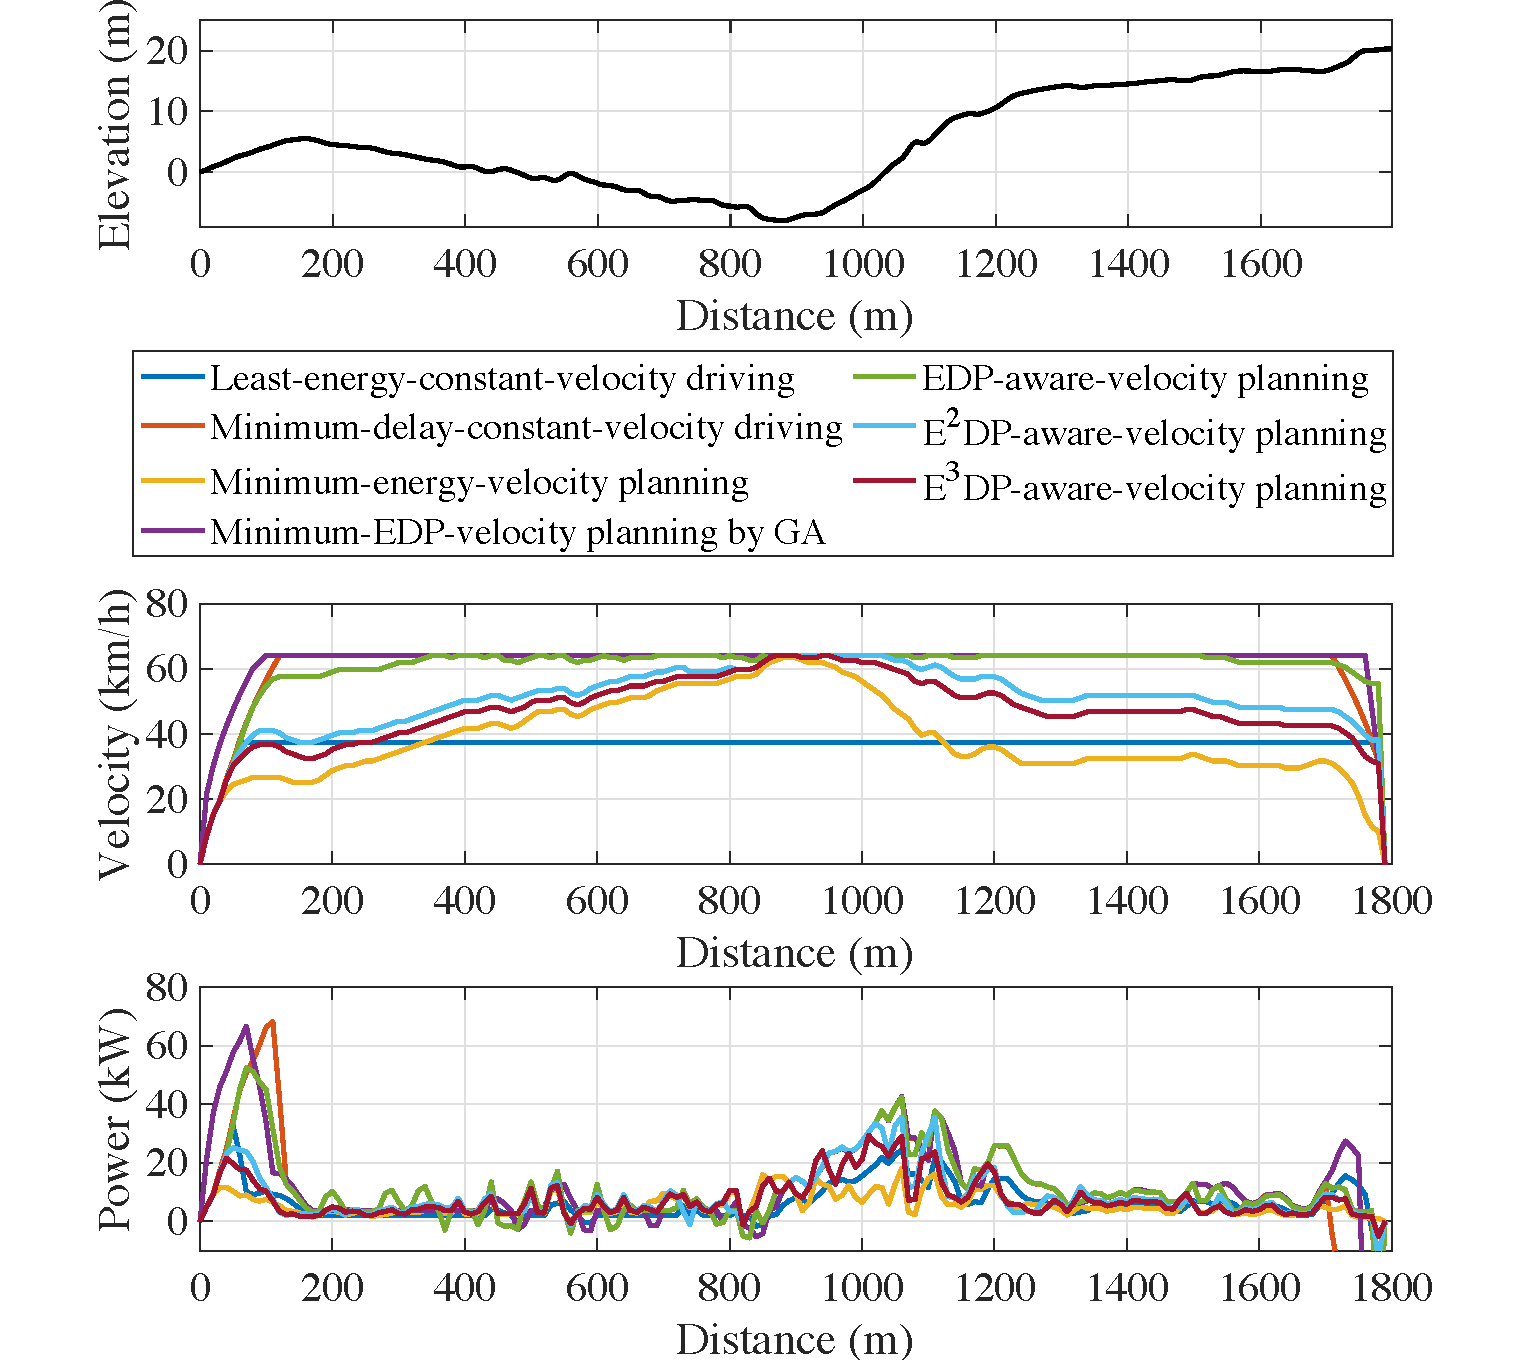
\includegraphics[width=\hsize]{Figures/EDP_comp_profile.pdf}
\caption{\textcolor{red}{Velocity profile comparison with cost functions of $EDP$, $E^2DP$ and $E^3DP$ on the benchmark Jones Street in San Francisco.}}
\label{fig:EDP_aware_velocity_planning}
\end{figure} 



\textcolor{red}{Fig.~\ref{fig:EDP_aware_velocity_planning} shows the $EDP$-aware-velocity planning result on road segments in a city (Cliff drive in Santa Barbara). We use the minimum-delay-constant-velocity driving and the least-energy-constant-velocity driving as baselines obtained by DSE. The minimum-energy-velocity planning and minimum-EDP-velocity planning by Genetic algorithm are used as golden references minimizing energy consumption and EDP, respectively.}
%
The minimum-energy-velocity planning, the least-energy-constant-velocity driving and minimum-delay-constant-velocity driving do reduce the $EDP$ but cannot explicitly minimize $EDP$. However, the $EDP$-aware-velocity planning often overrides the least-energy velocity because the delay penalty due to the reduced velocity is greater than the energy penalty due to the increased torque. Therefore, this policy can be used when the deadline is tight. Chances of energy saving by the energy-aware-velocity planning decrease as the deadline becomes tighter. 
%
The $EDP$-aware-velocity planning maintains the EV velocity to the least-energy velocity or the minimum-velocity constraint (not to bother traffic), whichever comes first. However, it does not appreciably decelerate the EV at the top of the hill to reduce driving time. So, we use $EDP$ for the metric when the deadline is tight. 

On the other hand, when the $E^2DP$ is used as a metric to optimize, the energy penalty contributes more to the cost function. As a result, the driving velocity decreases when driving on an uphill because the energy penalty due to the increased torque is greater than the delay penalty as shown in Fig.~\ref{fig:EDP_aware_velocity_planning}. Also, the $E^2DP$-aware velocity becomes slower than the maximum velocity on a downhill or on a flat road since the energy penalty becomes higher than the delay penalty at a high velocity due to the drivetrain loss and increased torque by the aerodynamic resistance. The EV accelerates to the least-energy velocity or the minimum-velocity constraint, whichever comes first, by the road slope and decelerates at the top of the first hill. Then, the EV drives faster than the least-energy velocity on the downhill followed by a  flat road, in preparation for the next hill. Although the least-energy velocity on an uphill is higher than that on a flat road, climbing an uphill consumes more energy. So, the EV gradually loses the velocity while it climbs up on an uphill spending less motor torque, which significantly saves energy consumption. In most applications, the deadline is important but not truly hard. Therefore, we adopt $E^2DP$ for the performance metric to consider both energy and driving time.

When it comes to $E^3DP$, the effect of energy penalty becomes even more distinct, and the average driving velocity becomes lower. 
The $E^3DP$ metric can be a proper optimization metric when the battery state of charge is less than 30\% for example.

%%Description for Fig. 12
Fig.~\ref{fig:EDP_bar} shows $EDP$ of the least-energy-constant-velocity driving, the minimum-delay-constant-velocity driving, the minimum-energy-velocity planning, the velocity planning with $EDP$, $E^2DP$ and $E^3DP$ as a metric on various road benchmarks \textcolor{red}{and the minimum-EDP-velocity planning with GA}. The proposed velocity planning results in up to 46.2\% improvements of $EDP$ compared with the least-energy-constant-velocity driving. 
%The improvements occur especially when the slope of the uphill is steep.
The driving velocity on a flat road is faster than that of the least-energy-constant-velocity driving at the expense of relatively little energy to save driving time. Then, the velocity decreases when climbing the following uphill to spend less motor torque, which saves more energy.

\textcolor{red}{In addition, the proposed EDP-aware-velocity planning is merely 4.3\% higher than the true EDP-minimum-velocity planning on average. Through this results, we confirm that the results of the proposed heuristics are close enough to the true optimal solutions.}


\begin{figure*}	 %Figure 12.
\centering
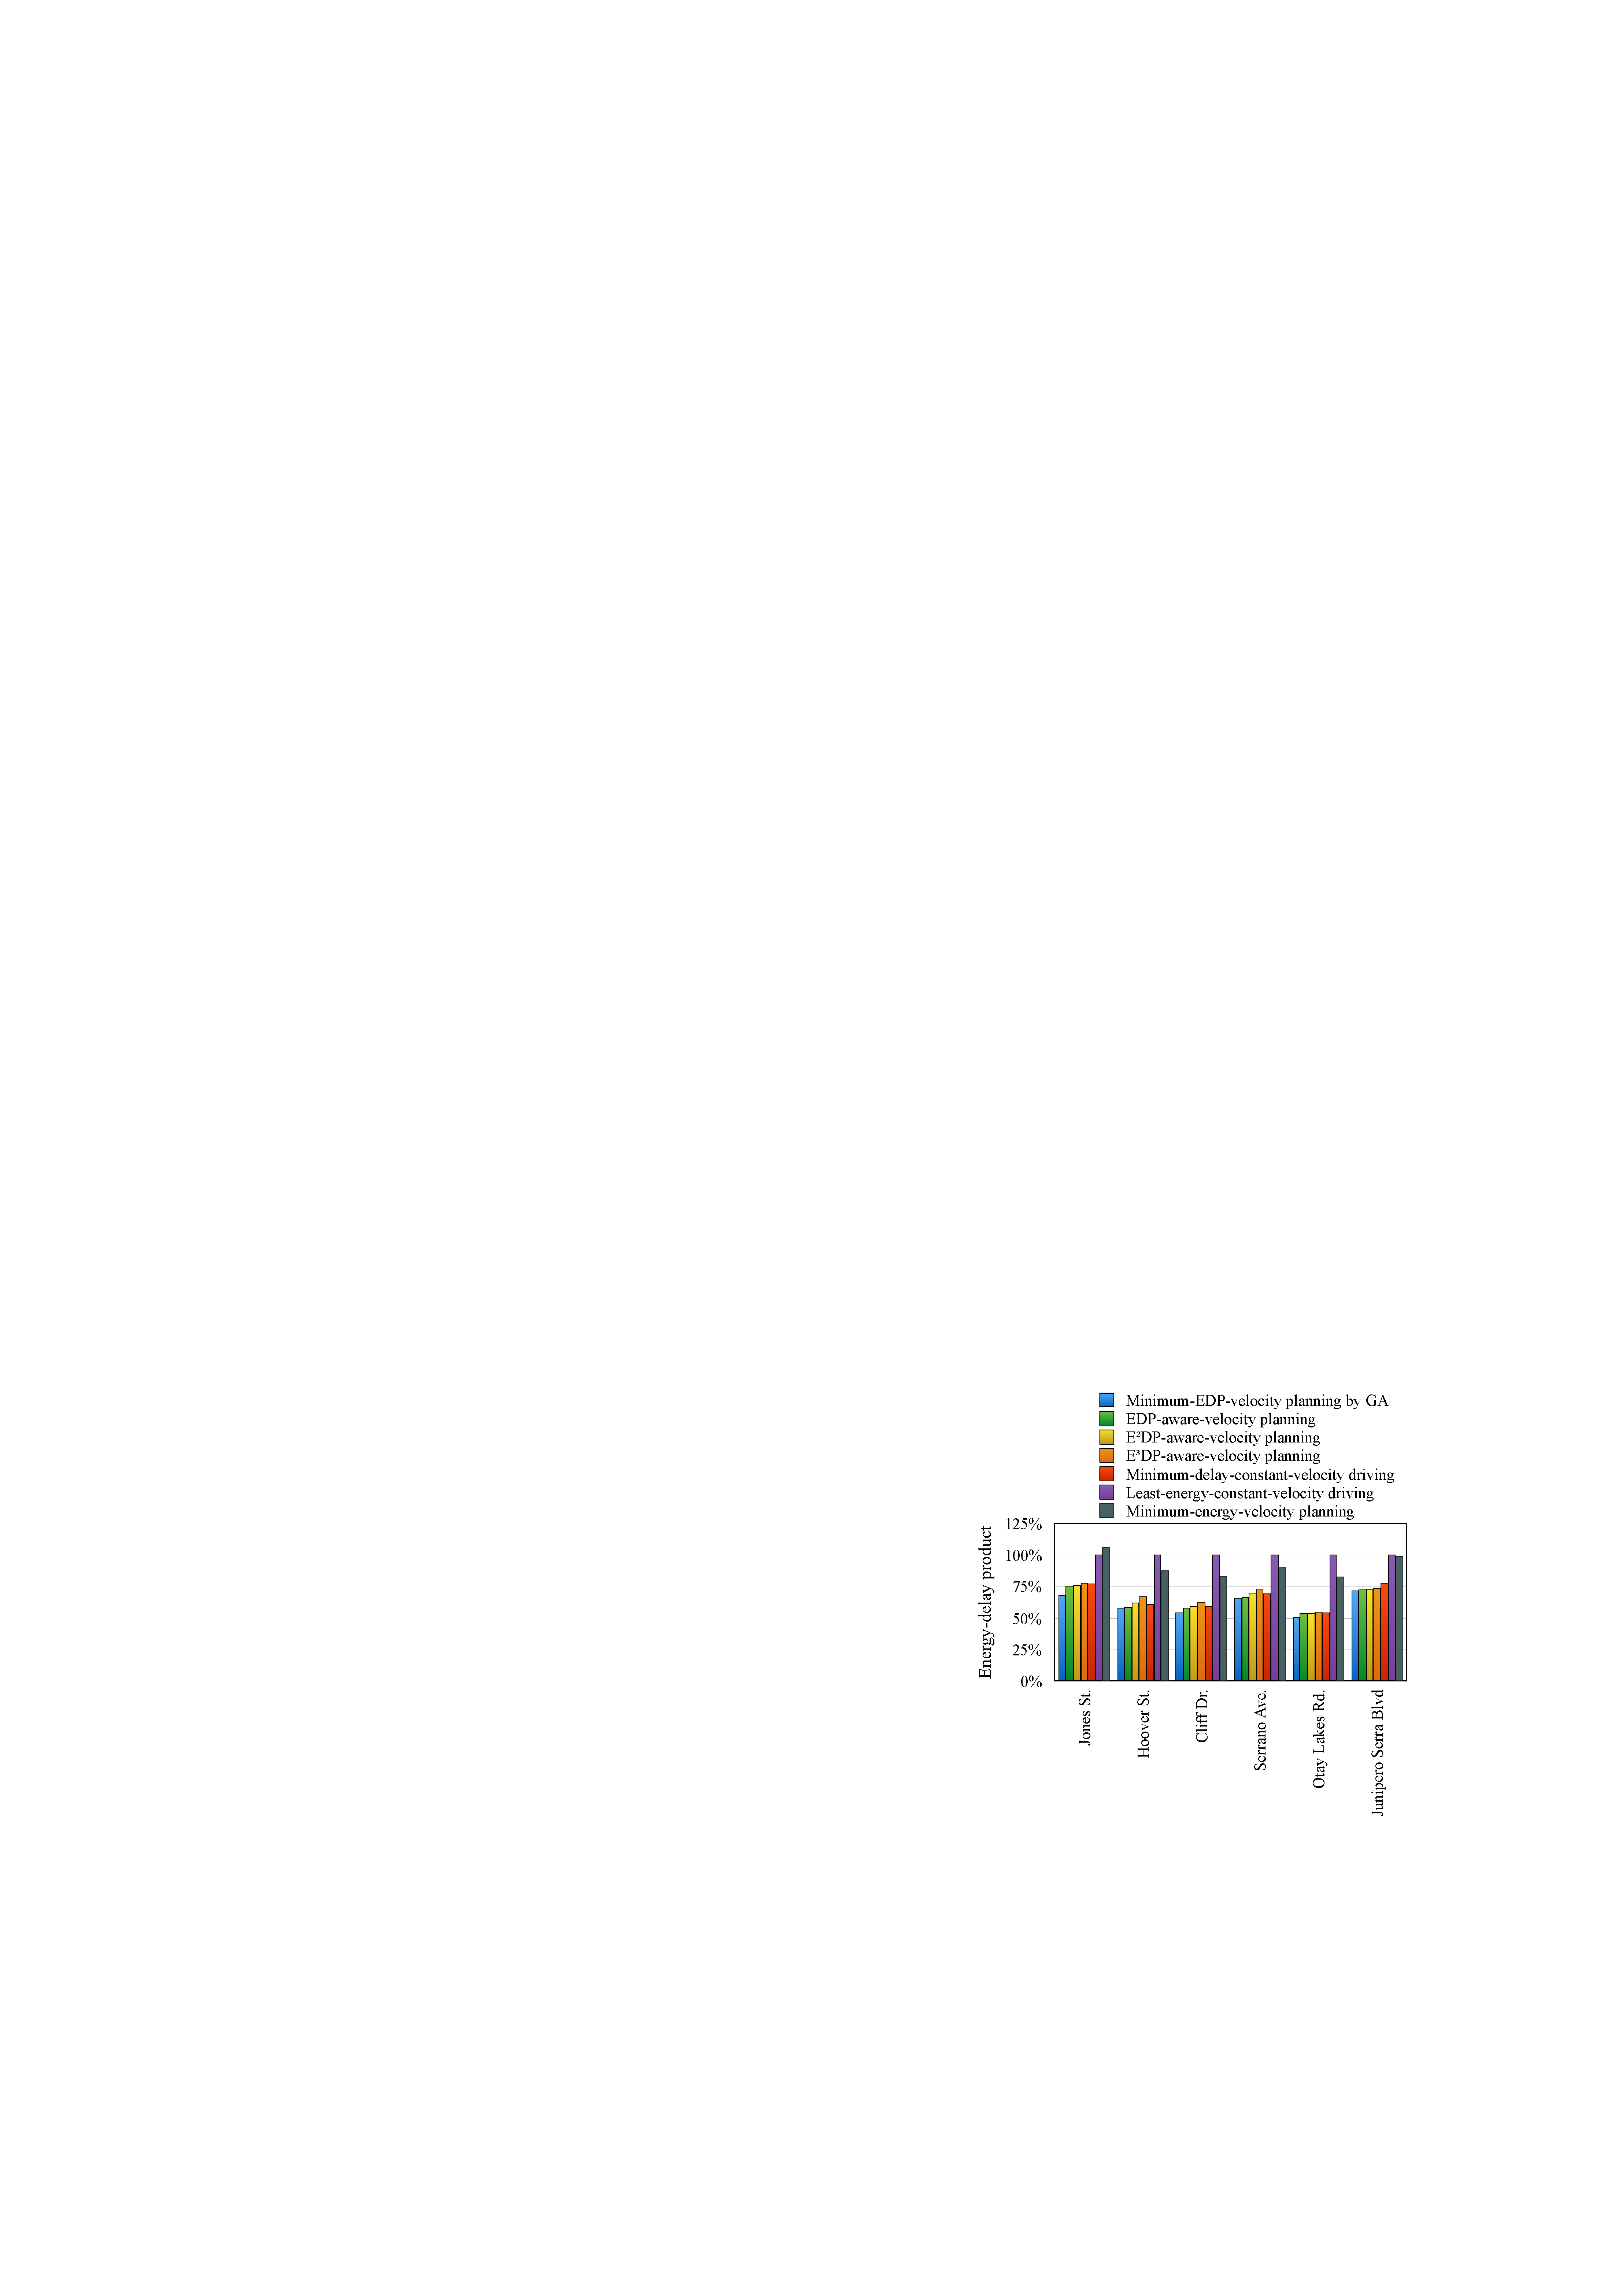
\includegraphics[width=\hsize]{Figures/EDP_comp_bar.pdf}
\caption{\textcolor{red}{Comparison of $EDP$ for various energy-aware-velocity planning methods.}}
\label{fig:EDP_bar}
\end{figure*} 


%Histogram analysis
\textcolor{red}{We quantize the velocity and acceleration values and make a histogram to analyze population of velocity and acceleration for various energy-aware-velocity planning methods. Fig.~\ref{fig:histogram} shows histogram of the driving schemes in Fig.~\ref{fig:EDP_aware_velocity_planning}. The minimum-delay-constant-velocity driving guides to accelerate to speed limit of the route benchmark (60 km/h). For the EDP-aware-velocity planning, it is used when the deadline is the most important concern. Therefore, it is also guided to drive near speed limit. The $E^2DP$- and $E^3DP$-aware-velocity planning methods are used when the remaining battery state of charge is more concerned than the deadline. It is guided to drive at an energy-efficient speed along a road slope. Particularly, the $E^3DP$-aware-velocity planning method is used when the state of charge is more concerned, and the driver should find the nearby charging station. It is guided to decelerate to 35-40 km/h.}

\begin{figure}	%Figure 13.
\centering
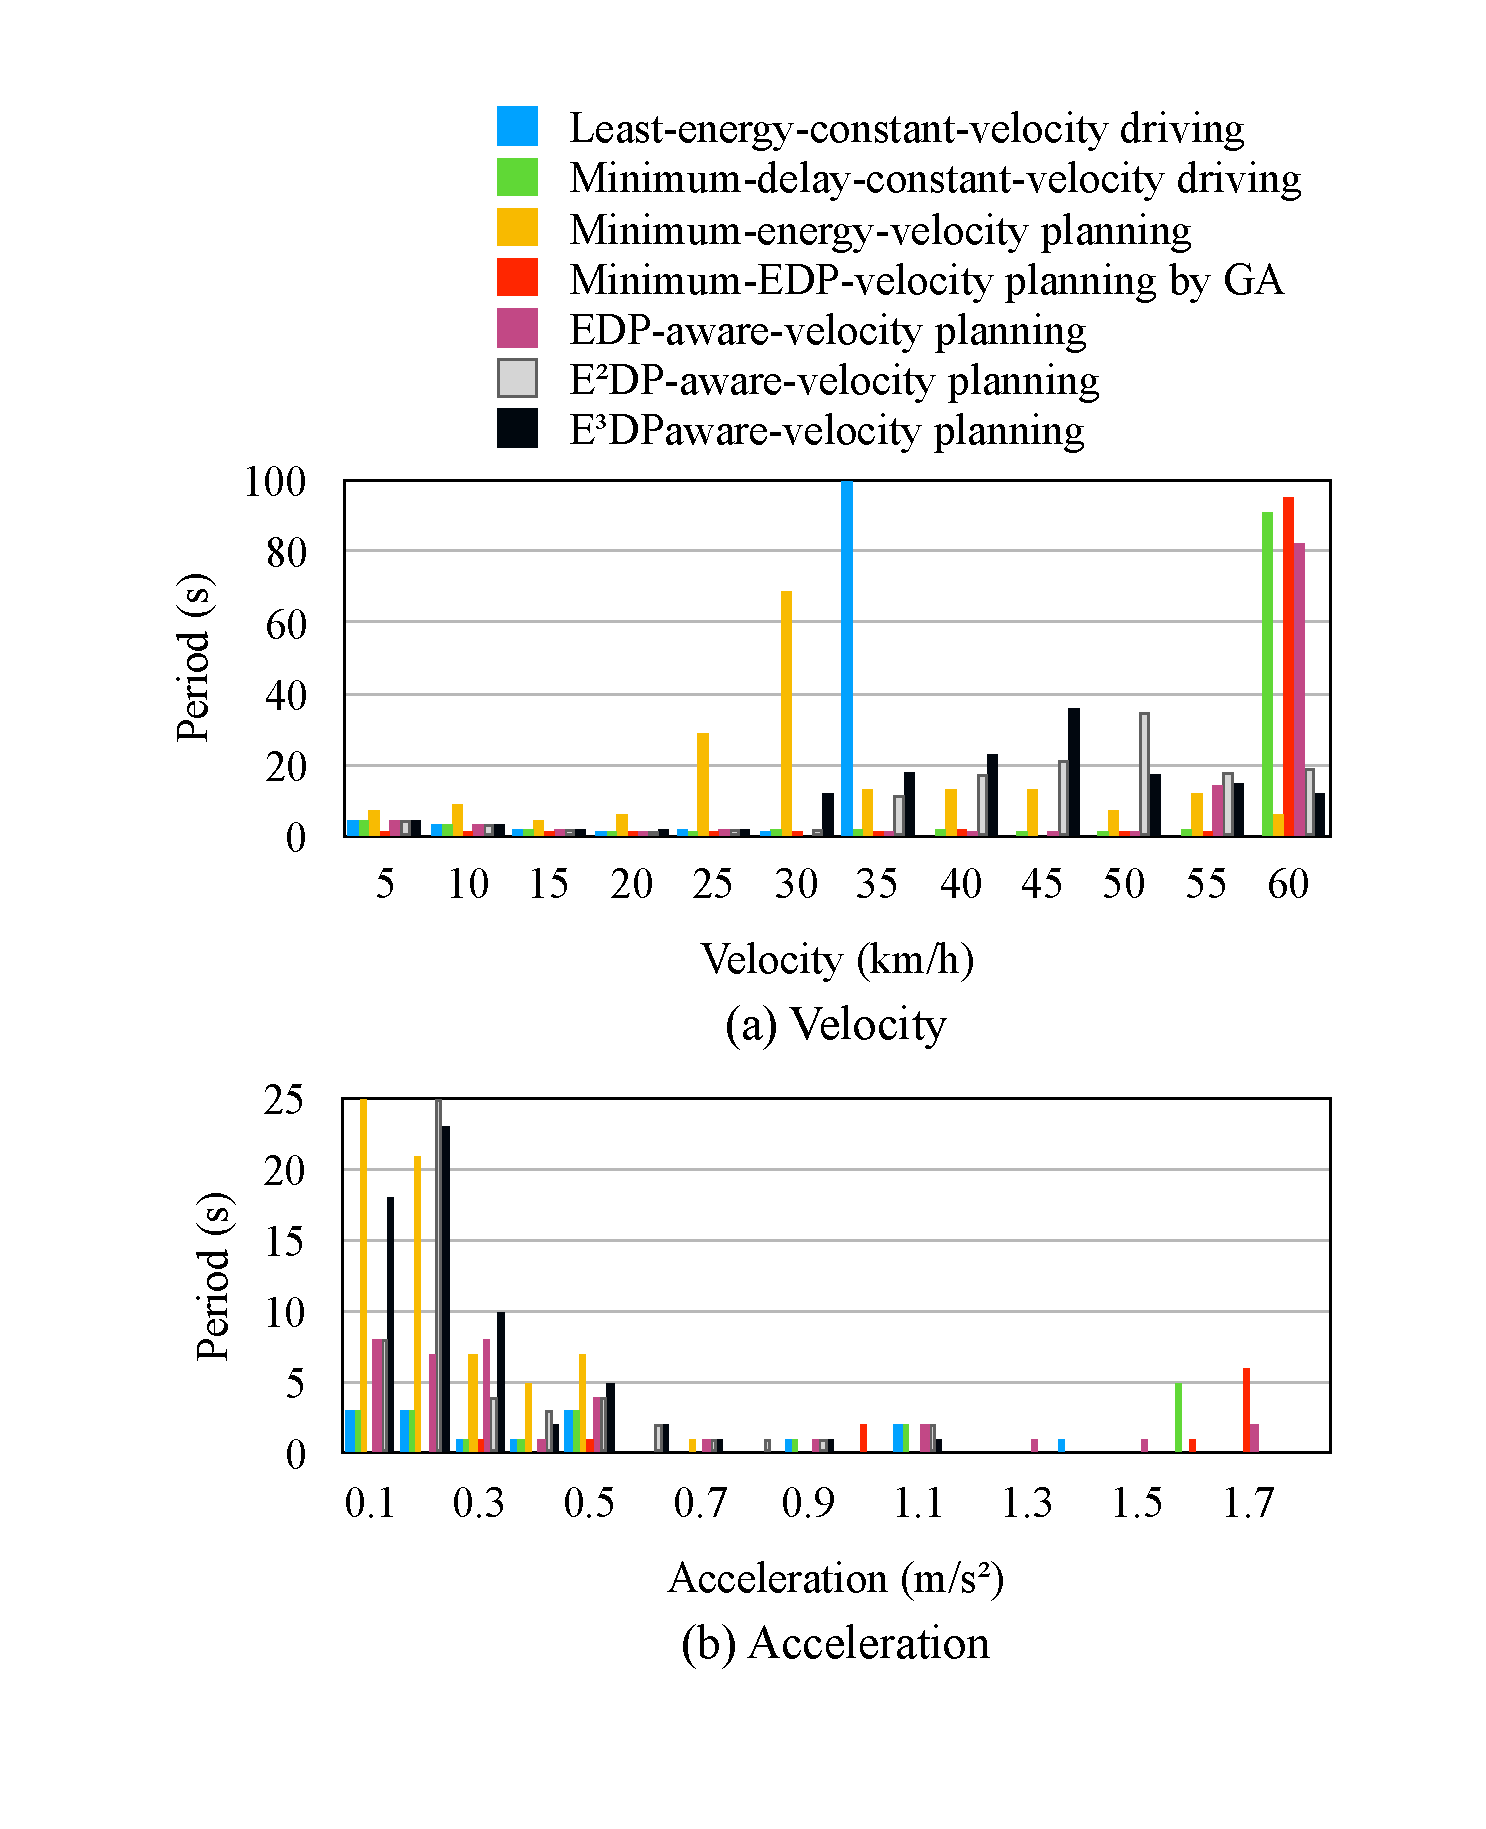
\includegraphics[width=\hsize]{Figures/Histogram.pdf}
\caption{\textcolor{red}{Histogram of (a) velocity and (b) acceleration for various energy-aware-velocity planning methods.}}
\label{fig:histogram}
\end{figure} 


%%%%%%%%%%%%%%%%%%%%%%%%%%%%%%%%%%%%%%%%%%
\section{Impact of the EV power model fidelity} \label{sec:impact_EV_power model}
%%%%%%%%%%%%%%%%%%%%%%%%%%%%%%%%%%%%%%%%%%

Lesson learned from embedded systems power management, it is crucial to extract an accurate power model from the device to system. Power optimization results largely change by the power model. Inaccurate power model obviously misleads the power optimization results. It goes without saying that an accurate EV power model mandates for the minimum energy velocity problem that reflects power variation by the velocity, acceleration, road slope, payload, and so forth.

%% Should be updated.
\begin{figure}	 %Figure 14.
\centering
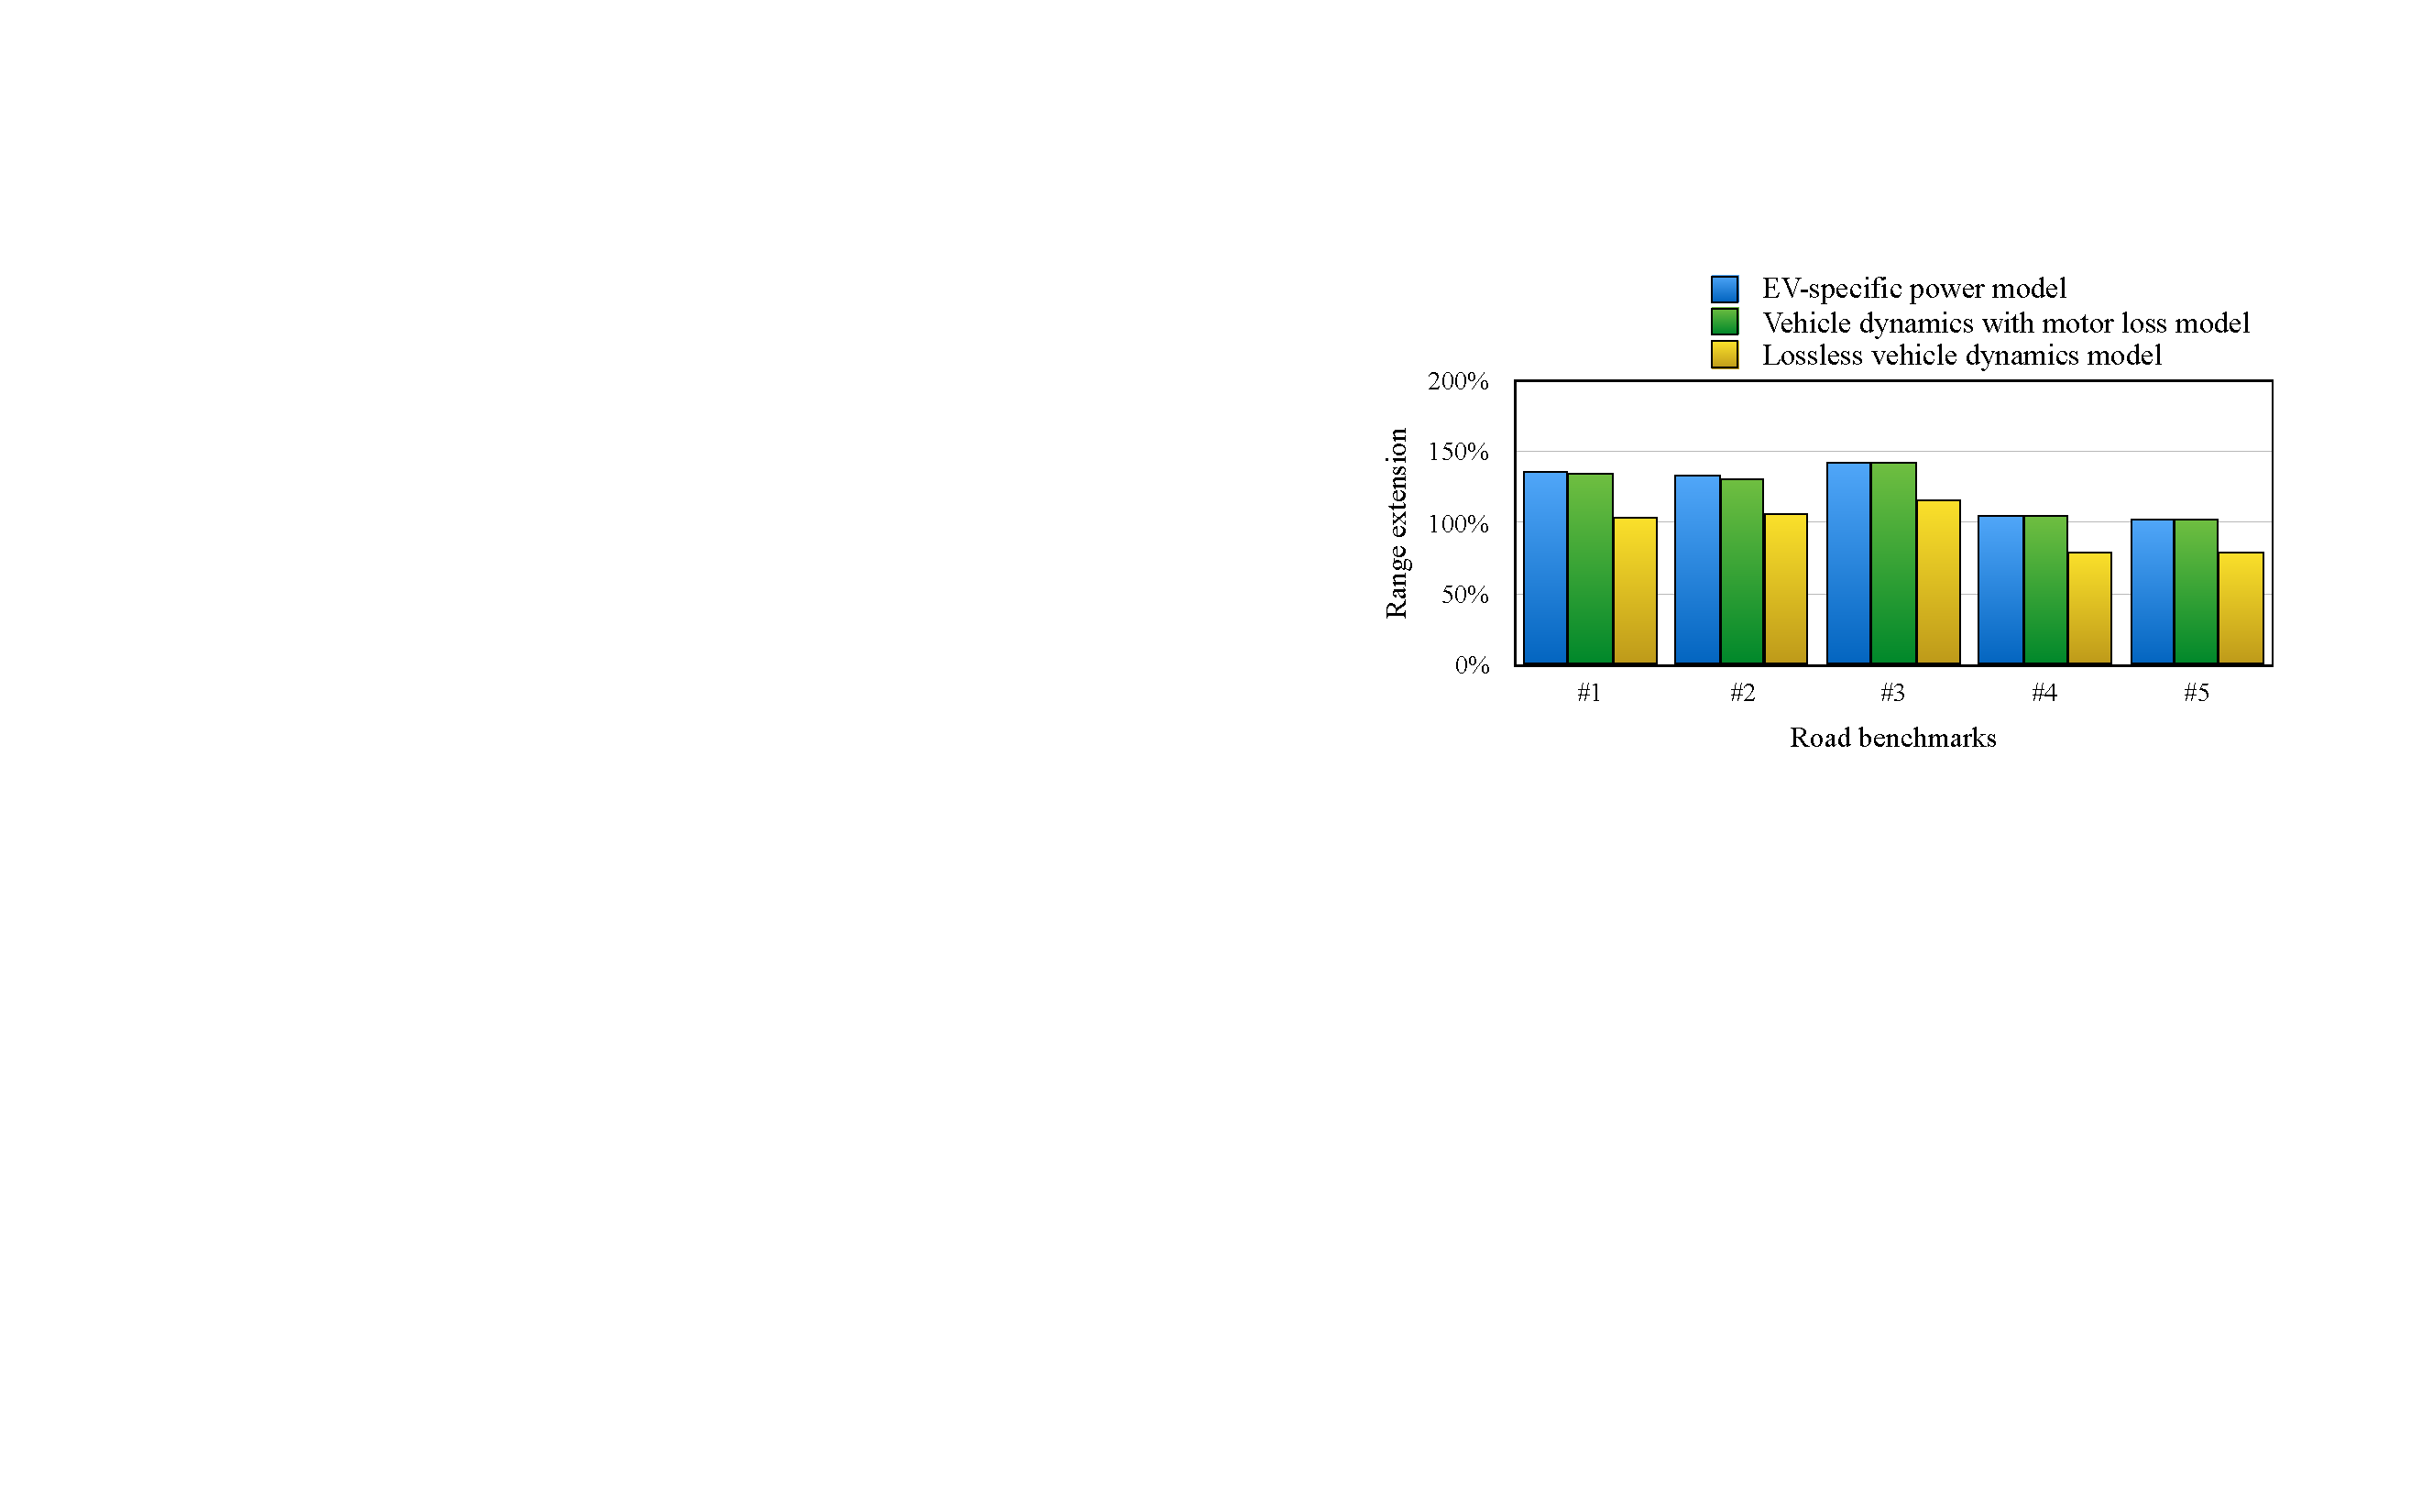
\includegraphics[width=\hsize]{Figures/model_fidelity.pdf}
%\caption{Range comparison by EV power consumption models.}
\caption{\textcolor{red}{Should be updated.}}
\label{fig:energy_by_model}
\end{figure} 

We compare the energy-aware-velocity planning results with i) a lossless vehicle dynamics model (\ref{eq:dynamics_model}), ii) a vehicle dynamics model with motor loss (\ref{eq:motorloss_model}) and iii) an EV-specific power model (\ref{eq:EV_specific_model}) described in Section~\ref{subsec:opt-cruising}. Inaccurate EV power consumption model causes suboptimal EV driving optimization.

Fig.~\ref{fig:energy_by_model} shows the comparison of range extension by the EV power models. The X-axis indicates the types of benchmark road slopes, and y-axis indicates the range; 100\%  range implies the range by the least-energy-constant-velocity driving. Blue-colored bars indicate the range with the EV-specific power model. Green and yellow-colored bars indicate the range with the vehicle dynamics with motor loss model and the lossless vehicle dynamics model, which does not consider motor loss and vehicle power loss at the drivetrain.

Driving optimization using more accurate power model shows more extended range. The extended range with the EV-specific power model is up to 4.0\% and 33.4\% compared with the minimum-energy-velocity planning with the vehicle dynamics with motor loss model and lossless vehicle dynamics model, respectively. One of the main reasons is that the underestimated EV power loss becomes a considerable portion of total energy consumption when the EV drives on low road slope or downhill.

%%%%%%%%%%%%%%%%%%%%%%%%%%%%%%%%%%%%%%%%%%
\section{Conclusions} \label{sec:conclusions}
%%%%%%%%%%%%%%%%%%%%%%%%%%%%%%%%%%%%%%%%%%

This paper introduces a novel energy-aware-velocity planning for battery electric vehicles (BEV or all-electric vehicles), which is inspired by low-power scheduling for computing systems. This work is a showcase such that classic system-level  low-power design methodologies significantly improves electric vehicle fuel efficiency. We demonstrate the potential gain from the proposed energy-aware-velocity planning for EV. We show the importance of EV-specific power model  comparing the actual energy gain from EV using different fidelity power models. In addition, this paper is the first to show the difference of the energy-aware-velocity planning between the full electric vehicles and internal combustion engine vehicles. Most importantly, we introduce energy and time combined metrics such as, energy-delay product ($EDP$), energy-square-delay product ($E^2DP$) and energy-cubic-delay product ($E^3DP$) for a tight time deadline constraint, a loose time deadline constraint, and a tight energy constraint, respectively. 
The proposed method results in up to a 43.4\% extended range and a  51.7\% improvement of the energy-delay product compared with the least-energy-constant-velocity driving. 
The energy-aware-velocity planning will become more crucial when full autonomous driving is widely deployed.


%%%%%%%%%%%%%%%%%%%%%%%%%%%%%%%%%%%%%%%%%%%
%\section*{Acknowledgment}
%%%%%%%%%%%%%%%%%%%%%%%%%%%%%%%%%%%%%%%%%%%

\bibliographystyle{ieeetr}
\bibliography{EV}

\begin{IEEEbiography}[{
\includegraphics[width=1in,height=1.25in,clip,keepaspectratio]{Bio/Donkyu.pdf}}]{Donkyu Baek}
(M'17) received the B.S. degree in Electrical Engineering from Hanyang University, Seoul, Korea, in 2009, and the M.S. and Ph.D. degrees from the Department of Electrical Engineering, Korea Advanced Institute of Science and Technology (KAIST), Daejeon, Korea, in 2011 and 2017, respectively. He is working with the Department of Electrical Engineering at KAIST in 2017 as a postdoctoral research fellow. 

Dr. Baek is the winner of the 2017 ISLPED Low-Power Design Contest Award (honorable mention) and the 2017 Design automation Conference Best University Demonstration Award (honorable mention.) He serves as an Information Director of the ACM Transactions on Design Automation of Electronics Systems (ACM TODAES.)
\end{IEEEbiography}

%Should be updated
%\begin{IEEEbiography}[{\includegraphics[width=1in,height=1.25in,clip,keepaspectratio]{Bio/Jaemin.jpg}}]{Jaemin Kim}
%\end{IEEEbiography}


\begin{IEEEbiography}[{
\includegraphics[width=1in,height=1.25in,clip,keepaspectratio]{Bio/Naehyuck.pdf}}]{Naehyuck Chang}
(F’12) received the B.S., M.S., and Ph.D. degrees from the Department of Control and Instrumentation, Seoul National University, Seoul, Korea, in 1989, 1992, and 1996, respectively. He was with the Department of Computer Science and Engineering, Seoul National University, from 1997 to 2014. He was an LG Yonam Foundation Research Professor in 2005. He served as a Vice Dean of the College of Engineering with Seoul National University from 2011 to 2013. He has been a Full Professor with the Department of Electrical Engineering, Korea Advanced Institute of Science and Technology, Daejeon, Korea, since 2014. His current research interests include low-power embedded systems and design automation of things, such as systematic design and optimization of energy storage systems and electric vehicles.

Dr. Chang is a fellow of the Association for Computing Machinery (ACM) for his contributions to low-power systems. He is the winner of the 2014 ISLPED Best Paper Award, 2011 SAE Vincent Bendix Automotive Electronics Engineering Award, 2011 Sinyang Academic Award, 2009 IEEE SSCS International SoC Design Conference Seoul Chapter Award, and several ISLPED Low-Power Design Contest Awards in 2002, 2003, 2004, 2007, 2012, 2014, and 2017. He is the editor-in-chief of the ACM Transactions on Design Automation of Electronics Systems (ACM TODAES) and serves(ed) as associated editor of IEEE TVLSI, IEEE TCAD, ACM TECS, IEEE ESL, IEEE TCAS-I, ACM TECS, etc. He served for the chair of ACM SIGDA (Special Interest Group on Design Automation) and is currently past chair of ACM SIGDA. He was TPC co-chair of DAC 2016, ASP-DAC 2015, ICCD 2014, CODES+ISSS 2012, ISLPED 2009, etc., and general co-chair of VLSI-SoC 2015, ICCD 2015 and 2014, ISLPED 2011, etc.


\end{IEEEbiography}


% that's all folks
\end{document}
